\documentclass[11pt]{article}
\pdfinfoomitdate=1
\pdftrailerid{}
\pdfsuppressptexinfo=15
\usepackage[T1]{fontenc}
\usepackage{lmodern}
\usepackage[expansion=false]{microtype}
\usepackage[margin=1.04in]{geometry}
\usepackage{amsmath,amssymb,amsthm,mathtools}
\usepackage{enumitem,booktabs,array,needspace}
\usepackage{tikz}
\usetikzlibrary{arrows.meta,positioning,calc,fit}
\usepackage[hyphens]{url}
\usepackage[hidelinks,hypertexnames=false]{hyperref}
\usepackage[nameinlink,capitalize,noabbrev]{cleveref}
\hypersetup{pdftitle={The Partition Principle does not imply Choice},pdfauthor={OpenAI}}
\setlength{\emergencystretch}{2em}
\allowdisplaybreaks[1]
\numberwithin{equation}{section}
\newtheorem{theorem}{Theorem}[section]
\newtheorem{lemma}[theorem]{Lemma}
\newtheorem{proposition}[theorem]{Proposition}
\newtheorem{corollary}[theorem]{Corollary}
\theoremstyle{definition}
\newtheorem{definition}[theorem]{Definition}
\theoremstyle{remark}
\newtheorem{remark}[theorem]{Remark}
\newcommand{\ZF}{\mathsf{ZF}}
\newcommand{\ZFC}{\mathsf{ZFC}}
\newcommand{\AC}{\mathsf{AC}}
\newcommand{\PP}{\mathsf{PP}}
\newcommand{\ACwo}{\mathsf{AC}_{\mathrm{WO}}}
\newcommand{\Con}{\operatorname{Con}}
\newcommand{\Ord}{\mathrm{Ord}}
\newcommand{\HS}{\mathrm{HS}}
\newcommand{\forces}{\Vdash}
\DeclareMathOperator{\Fix}{Fix}
\DeclareMathOperator{\Sym}{Sym}
\DeclareMathOperator{\dom}{dom}
\DeclareMathOperator{\ran}{ran}
\DeclareMathOperator{\supp}{supp}
\DeclareMathOperator{\id}{id}
\title{The Partition Principle does not imply Choice}
\author{OpenAI}
\date{September 24, 2026}
\begin{document}
\maketitle
\begin{abstract}
We prove that the Partition Principle does not imply the Axiom of Choice:
if ZF is consistent, then so is ZF with the Partition Principle, Choice for
ordinal-indexed families, and the negation of the Axiom of Choice.
Separately, over every countable transitive model of ZFC, we construct a
transitive symmetric model of this theory with the same ordinals and no new
countable sequences of ground elements.
\end{abstract}
\tableofcontents
\clearpage
\section{Introduction}\label{sec:introduction}

The \emph{Partition Principle} asserts that a surjection between two sets
implies the existence of an injection in the reverse direction:
\[
 \PP:\qquad
 \forall X\,\forall Y\,
 \bigl[(\exists f:X\twoheadrightarrow Y)
       \Longrightarrow(\exists j:Y\hookrightarrow X)\bigr].
\]
Equivalently, every partition of a set admits an injection into that set.
The Axiom of Choice implies this principle by choosing one element of each
fiber. The converse is less direct: the injection supplied by $\PP$ need
not take a part to one of its members. In particular, it need not satisfy
$f\circ j=\id_Y$. The problem is whether this cardinal comparison alone
can recover choice for arbitrary families.

Write $\ACwo$ for Choice for wellorderable families: for every ordinal
$\eta$ and every family $(X_\xi)_{\xi<\eta}$ of nonempty sets, there is a
function $c$ with $c(\xi)\in X_\xi$ for all $\xi<\eta$.
Our principal result is the following ordinary relative-consistency statement.

\begin{theorem}\label{thm:main-consistency}
If $\ZF$ is consistent, then so is $\ZF+\PP+\ACwo+\neg\AC$.
\end{theorem}

The construction also has a separate transitive-model form.

\begin{theorem}\label{thm:main-transitive}
Let $V$ be a countable transitive model of $\ZFC$. There are a set forcing
$\mathbb Q\in V$, a $V$-generic filter $G$, and a transitive symmetric
submodel $W$ of $V[G]$ such that
\[
 V\subseteq W\subseteq V[G],\qquad
 \Ord^W=\Ord^V,\qquad
 W\models\ZF+\PP+\ACwo+\neg\AC.
\]
Every countable sequence of elements of $V$ that belongs to $W$ already
belongs to $V$.
\end{theorem}

Here $\ZF$ is classical first-order set theory with pure sets, Foundation,
and the full Separation and Replacement schemata.
Theorem~\ref{thm:main-consistency} gives a negative answer to the
Partition Principle versus Choice problem under ordinary syntactic
consistency. It permits externally ill-founded models, whereas
Theorem~\ref{thm:main-transitive} starts with a transitive ground and
preserves transitivity. In either conclusion the reverse injections and
the family without a choice function belong to the same model.
Section~\ref{sec:metatheory} gives the two deductions separately.
The consequences for the dual Cantor--Schr\"oder--Bernstein principle
and the Weak Partition Principle are developed in
Remark~\ref{rem:dual-csb-wpp}.

\subsection{History and related methods}

The distinction between comparing the sizes of a partition and its
underlying set, and actually choosing representatives, is longstanding.
Da Silva traces the Partition Principle
to Beppo Levi in 1902 \cite[Section~2, p.~787]{daSilva2021}.
Banaschewski and Moore studied its relation to the dual
Cantor--Bernstein theorem and the surrounding cardinal-comparison
principles \cite{BanaschewskiMoore1990}. These questions concern what
remains of cardinal arithmetic when sets need not be wellorderable.
For example, Blass and Kulshreshtha distinguish several forms of
cardinal well-foundedness and show that they become equivalent under
$\PP$; their August 2026 version still lists $\PP\Rightarrow\AC$
as open \cite[Introduction and Section~9]{BlassKulshreshtha2026}.
Gilson's September 2026 corrections withdraw the model-construction
claims of three earlier approaches
\cite{GilsonSheafCorrection2026,GilsonExternalCorrection2026,GilsonIterationCorrection2026}.

There is already substantial choice in $\PP$. The implication
$\PP\Rightarrow\ACwo$ is classical: Ryan-Smith records the
argument attributed to Pincus by Pelc
\cite[Proposition~3.17, proof and footnote~4]{RyanSmith2025}.
Thus $\ACwo$ in our main statements is not an additional strength
beyond $\PP$. Its separate appearance records the order of the
construction: we establish ordinal-indexed choice first and then use
it to assemble reverse injections for arbitrary sets.

The difficulty of preserving a principle quantified over all sets
can be reduced to a fixed set of parameters. Blass introduced small
violations of choice \cite{Blass1979}. For a nonempty set $A$,
$\mathrm{SVC}(A)$ says that every nonempty set is a surjective image
of $A\times\eta$ for some ordinal $\eta$. The injective version,
$\mathrm{SVC}^{+}(A)$, says that every set embeds into some
$A\times\eta$. See also
\cite[Definition~3.13 and Theorem~3.14]{Usuba2021}.
These presentations let a construction on one set control objects
of arbitrary rank, but their different directions cannot be
interchanged without proof.

Ryan-Smith makes the local-to-global step precise. Under
$\mathrm{SVC}^{+}(A)$, full $\PP$ is equivalent to $\ACwo$
together with reverse injections for surjections between subsets of
$A$ \cite[Proposition~3.17]{RyanSmith2025}. Reverse injections for
surjective images of $A$ are a different local assertion: even with
$\ACwo$ and $\mathrm{SVC}^{+}(A)$, they need not imply full
$\PP$ \cite[Proposition~3.23]{RyanSmith2025}. Our construction
instead makes every nonwellorderable image of $A$ bijective to $A$.
Lemma~\ref{lemma:pp-reduction} uses this stronger classification,
the surjective presentation, and ordinal-indexed choice to carry out
the required all-set reduction. Its slicing argument follows the
method of \cite[Propositions~3.17 and~3.20]{RyanSmith2025}, rather
than identifying the two local principles.

The ambient method is a symmetric submodel of a set-forcing
extension: hereditarily symmetric names for a normal filter of
subgroups give a model of full $\ZF$
\cite[Section~2.1]{Karagila2026}. A more specific antecedent is
Holy and Schilhan's product of Cohen forcing with a forcing of
ground-model hereditarily almost-disjoint towers
\cite[Section~3]{HolySchilhan2025}. Their construction yields
models in which every set can be linearly ordered and higher forms
of Dependent Choice hold, although full Choice fails. They develop
the hereditary almost-disjointness method from Pincus's work on
adding Dependent Choice \cite{Pincus1977}. Their restriction and
support-intersection arguments
\cite[Lemmas~10 and~15]{HolySchilhan2025} are antecedents of the
locality arguments here. Our diagrams have a different geometry:
the monoid must support both exact quotient multiplicities and the
coherent assignment of bijections, not just the descent of supports.

\subsection{Proof strategy}

We construct a set $A$ of distinct generic subsets of the ground-model
$\omega_1$. Symmetry
prevents $A$ from being wellordered. Orbit maps of names show that every
nonempty set is a surjective image of $A\times\eta$ for some ordinal
$\eta$, with no restriction on its rank. The forcing also allows one
wellorderable part of $A$ to meet every member of any given ordinal-indexed
family of nonempty subsets of $A$. Together with the preceding
presentation of arbitrary sets, this yields $\ACwo$.

The central additional property is
\begin{equation}\label{eq:intro-quotient}
 \text{every nonwellorderable surjective image of $A$ is in bijection with $A$.}
\end{equation}
To pass from this property to full $\PP$, partition the target of an
arbitrary surjection into ordinal-indexed disjoint nonempty pieces and
use disjoint source pieces mapping onto them. Each resulting piece is
an image of $A$, though the source pieces need not cover the original
domain. A wellorderable target piece admits a reverse injection by
$\ACwo$. Otherwise both corresponding pieces are in bijection with $A$
by \eqref{eq:intro-quotient}. A further application of $\ACwo$ chooses
the piecewise injections, whose union is the required injection. The
empty target uses the empty injection.

The difficult part is to construct the bijections in
\eqref{eq:intro-quotient} with enough coherence to belong to the symmetric
model. Fix one equivalence relation on $A$ whose quotient is not
wellorderable. Counting its classes on
each support will produce many possible local bijections, but arbitrary
choices of them need not agree on overlapping supports or respect
coordinate changes. The proof solves these two compatibility problems
in three stages.

\begin{enumerate}[leftmargin=*,label=\arabic*.]
\item \textbf{A geometry of diagrams.}
We build a left-cancellative monoid $T$. A diagram is an injective map
$r:T\to I$, where $I$ is the set of label indices. Its subdiagram at $n\in T$
is the map $r_n(x)=r(nx)$. The diagram forcing makes larger diagrams
stronger conditions. Finite amalgamations join independently placed
diagrams. A second extension operation places many copies with prescribed
patterns of intersection. Together these operations give the forcing its
compatibility and support-descent properties. Height and cost functions
reduce the availability patterns introduced next to countable cofinal
paths. A rearrangement of the same monoid construction will later bound
the symmetries that survive along such a path.

\item \textbf{Exact availability fibers.}
A diagram supports names whose definitions are fixed by all permutations
of labels outside its range. For a quotient of $A$, we record the quotient
elements that can be named at each diagram. An element's availability
pattern records the subdiagrams at which it can still be named.
The labels themselves have analogous patterns, determined by which
subdiagrams contain their indices. The copying and support-descent lemmas
show that, for each exact pattern, the available labels and quotient
elements have the same cardinality. Restricting to a subdiagram in that
pattern identifies the corresponding fibers canonically. These
identifications group the fibers into components and are already
compatible; the choices of bijections between label and quotient fibers
are not.

\item \textbf{Covariant choices on each component.}
Each component has a countable cofinal chain of nested diagrams. Codes
along this chain give a preliminary bijection compatible with every
permutation fixing a sufficiently late diagram pointwise. Modulo these
permutations, the remaining symmetries form a countable group. Countably
many bounded initial segments of Cohen subsets distinguish its elements
and select among the transported preliminary bijections. Finally,
transport between components gives assignments that agree under
restriction and respect all required permutations. Their union is one
hereditarily symmetric graph for the fixed quotient.
\end{enumerate}

The countable description of each availability pattern, the reduction of
its symmetries to a countable group, and the final equivariant selection
are the main technical ingredients. The selection is performed between
moved Cohen generics: it does not require permutations to act as
automorphisms of a single fixed forcing extension.

Section~\ref{sec:monoid} constructs $T$ and proves its local rearrangement
property. Section~\ref{sec:forcing} develops the forcing, locality, and the
basic properties of $A$. The quotient construction follows in
three stages: Section~\ref{sec:quotient-fibers} computes exact availability
fibers, Section~\ref{sec:quotient-components} organizes them into components
and controls their symmetries, and Section~\ref{sec:quotient-equivariance}
constructs the coherent bijections. Section~\ref{sec:conclusion} derives
full $\PP$ and identifies a family without a choice function.
Section~\ref{sec:metatheory} gives the ordinary consistency deduction and
the separate transitive-ground result.

\section{A monoid of diagrams}\label{sec:monoid}

The forcing construction will compare a diagram with its translated
subdiagrams.  We first construct the monoid that indexes these
translations.  Its two extension operations serve different purposes:
one realizes finitely many prescribed overlaps, and the other inserts
many new positions with a prescribed set of old divisors.  A further
property of the construction will control symmetries along countable
systems of subdiagrams.

All constructions in this section take place in a universe satisfying
$\ZFC$.  No inaccessible cardinal is used.  Fix an infinite cardinal
$\mu\geq\aleph_1$ such that $\mu^{\aleph_0}=\mu$.

\subsection{The required algebra and the construction theorem}

Let $M$ be a monoid with identity $1$. Write $x\sqsubseteq y$ if $xz=y$ for
some $z$.  We use only left cancellation.  A monoid is \emph{conical}
if $xy=1$ implies $x=y=1$.  Left cancellation and conicality make
$\sqsubseteq$ a partial order and make the right factor in a comparison
unique.  Write $x\sqsubset y$ for $x\sqsubseteq y$ and $x\ne y$,
and $\downarrow a=\{x:x\sqsubseteq a\}$.
A \emph{conditional join} is an element $x\vee y$ satisfying
\[
 xM\cap yM=(x\vee y)M
\]
whenever the intersection is nonempty.  Thus a join is required exactly
when the two elements have a common right multiple.
An \emph{ideal} in $\downarrow a$ will mean a nonempty downward closed
subset closed under finite nonempty joins.  These joins exist because
$a$ is an upper bound.

An inclusion $B\subseteq M$ is \emph{conservative} if it preserves and
reflects comparisons, preserves their right factors, preserves existing
joins, and preserves the absence of a common right multiple.  In
particular, if $x,y\in B$ and $xz=y$ in $M$, then $z\in B$ and the
same equation holds in $B$.  Mere injectivity is not this property.

We shall also keep real-valued height and cost functions $\rho,\epsilon$
on $M$, writing $\epsilon_x=\epsilon(x)$, and satisfying
\begin{equation}\label{eq:mono-margin}
 \begin{gathered}
 0<\rho(x)<1,\qquad 0<\epsilon_x\leq1,\\
 \rho(y)-\rho(x)>
 \sup\{\epsilon_d:d\sqsubseteq y,\ d\not\sqsubseteq x\}
 \qquad(x\sqsubset y).
 \end{gathered}
\end{equation}
An empty supremum of costs is understood to be zero.

\begin{lemma}\label{lem:mono-countable-ideal}
If a monoid has conditional joins and satisfies
Equation~\eqref{eq:mono-margin}, every ideal in $\downarrow a$ has a
nondecreasing cofinal sequence of length $\omega$, with repetitions
allowed.  The same conclusion holds in any $\ZFC$ extension in which
the monoid, order, heights and costs retain their meanings, for ideals
belonging to that extension.
\end{lemma}
\begin{proof}
For an ideal $U$, choose elements whose heights approach
$\sup\rho[U]$, and replace their successive initial segments by their
finite joins.  This gives a nondecreasing sequence $(n_i)$ in $U$
with heights approaching the same supremum.  If $d\in U$ divides
none of the $n_i$, then
\[
 \rho(n_i\vee d)-\rho(n_i)>\epsilon_d
\]
for every $i$, contradicting convergence to the supremum.  Prepending
$1$ makes $n_0=1$.  The proof applies in the stated extension as well;
its choices are made in that $\ZFC$ universe.
\end{proof}

Here is the finite overlap condition used below.  Take finitely many
copies $\{i\}\times M$.  For each pair of distinct copies prescribe
either no overlap or elements $a_{ij},a_{ji}\in M$ and the
identifications
\[
 (i,a_{ij}x)\sim(j,a_{ji}x)\qquad(x\in M).
\]
We call the prescription \emph{valid} if these pair identifications,
together with equality, already form an equivalence relation and do
not identify distinct elements of any one copy.  In particular,
transitive closure is not allowed to create extra overlaps.

\begin{theorem}\label{thm:monoid}
There is a monoid $T$ of cardinality $\mu$, with a distinguished
$e\ne1$, having the following properties.
\begin{enumerate}
\item $T$ is left cancellative and conical, has conditional joins,
and has heights and costs satisfying Equation~\eqref{eq:mono-margin}.
\item Every valid finite overlap prescription on copies of $T$ is
realized by left translations $x\mapsto l_i x$ in $T$, with exactly
the prescribed identifications.
\item For $a,b\in T$ with $b\ne1$, and every ideal
$U\subseteq\downarrow a$, there are $\mu$ distinct elements $m$ with
\begin{equation}\label{eq:mono-probes}
 \begin{gathered}
 mb=ae,\qquad m\not\sqsubseteq a,\qquad
 \downarrow m\cap\downarrow a=U,\\
 n\vee m=ae\quad(n\sqsubseteq a,\ n\notin U).
 \end{gathered}
\end{equation}
The cones of distinct elements in this family intersect exactly in
$aeT$.  Moreover $|T\setminus eT|=\mu$.
\item For every countable subset of $T$ there is a countable
submonoid $T_0$ containing it and a continuous conservative tower
starting at $T_0$ and ending at $T$.  Each successor step has one of
the following properties:
\begin{enumerate}
\item no new element divides an old element;
\item every new element $w$ with an old right multiple has a least
old right multiple $g(w)$, and
\begin{equation}\label{eq:mono-gate-old}
 d\text{ old},\quad g(w)\sqsubseteq wd
       \quad\Longrightarrow\quad wd\text{ old}.
\end{equation}
\end{enumerate}
Here ``old'' means belonging to the base of that particular successor
step, and the comparisons may be tested in the final monoid.
\end{enumerate}
\end{theorem}

For diagrams indexed by $T$, the finite-merger clause supplies a common
larger diagram for finitely many copies with compatible overlaps.  The
probe clause supplies $\mu$ copies with one prescribed intersection
pattern: for $n\sqsubseteq a$, the cone $nT$ contains $mT$ exactly when
$n\in U$, and otherwise meets it in $aeT$.  The margin makes every such
ideal countably cofinal.  The countable-base clause serves a different
purpose: it will allow suitably extendible positions below a countable
path to be moved into a countable submonoid.  We formulate that descent
precisely at the end of the section and use it to bound the residual
symmetries of diagrams.

We prove the theorem through two extension lemmas.  They preserve more
than the order: keeping right factors and nonjoins fixed is what permits
the operations to be rearranged over a countable submonoid.

\subsection{The extension that inserts a probe}

Suppose $M$ has all the algebraic and margin properties above.
Fix $a,b,e\in M$, with $b,e\ne1$, and a nondecreasing path
\begin{equation}\label{eq:mono-path}
 1=n_0\sqsubseteq n_1\sqsubseteq\cdots\sqsubseteq a,
 \qquad n_id_i=n_{i+1},\qquad n_ic_i=a.
\end{equation}
Left cancellation gives $d_ic_{i+1}=c_i$.
Form the monoid presentation over $M$ with new generators $p_i$ and
relations
\begin{equation}\label{eq:mono-probe-relations}
 p_i=d_ip_{i+1},\qquad p_ib=c_ie\qquad(i<\omega).
\end{equation}
Put $m=p_0$.  Since $n_0=1$ and $n_id_i=n_{i+1}$, the first
relations give $n_ip_i=m$ for every $i$.  Thus every point of the path
divides the new probe.  The second relations make both factorizations
in Figure~\ref{fig:probe-divisibility} end at $ae$:
\[
 n_ip_ib=n_ic_ie=ae,\qquad mb=ae.
\]
These identities explain the presentation, but do not yet establish
its exact divisor profile.  We must prove that no old divisor of $a$
outside the path's downward closure is inserted below $m$, that $m$
does not divide $a$, and that every omitted divisor meets $m$ first
at $ae$.  The next lemma proves these
claims even for new divisors of $a$ introduced by the same extension.

\begin{figure}[htbp]
\centering
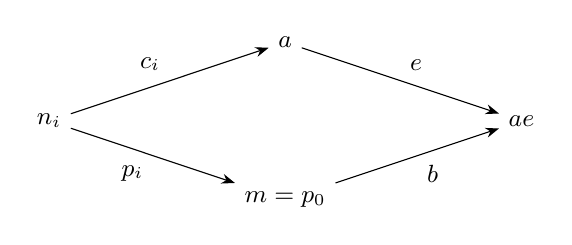
\begin{tikzpicture}[font=\small,>=Stealth]
  \node (pathpoint) at (0,0) {$n_i$};
  \node (oldpoint) at (3,1) {$a$};
  \node (probe) at (3,-1) {$m=p_0$};
  \node (commonmultiple) at (6,0) {$ae$};
  \draw[->] (pathpoint) -- node[above left] {$c_i$} (oldpoint);
  \draw[->] (pathpoint) -- node[below left] {$p_i$} (probe);
  \draw[->] (oldpoint) -- node[above right] {$e$} (commonmultiple);
  \draw[->] (probe) -- node[below right] {$b$} (commonmultiple);
\end{tikzpicture}
\caption{The relations defining the probe give two factorizations of
the prescribed common multiple $ae$.  Each arrow means right
multiplication by its label, not a covering relation.  This is not a
Hasse diagram: path points may coincide with $a$, and $a$ may divide
$m$.  The exact-profile assertion is that a divisor of $a$ omitted
from the path's downward closure has join $ae$ with $m$.}
\label{fig:probe-divisibility}
\end{figure}


\begin{lemma}\label{lem:mono-probe-algebra}
The presented extension $M'$ is left cancellative and conical, has
conditional joins, and conservatively contains $M$.  Every new element
with an old right multiple has a least old right multiple, and
Equation~\eqref{eq:mono-gate-old} holds at this extension.
For $m=p_0$,
\begin{equation}\label{eq:mono-probe-profile}
 \begin{gathered}
 mb=ae,\qquad m\not\sqsubseteq a,\qquad
 \downarrow m\cap\downarrow a=\bigcup_i\downarrow n_i,\\
 x\vee m=ae\qquad
 (x\sqsubseteq a,\ x\not\sqsubseteq m),
 \end{gathered}
\end{equation}
where the downsets and joins in this display are computed in $M'$.
\end{lemma}

\begin{proof}
\smallskip\noindent\textit{Normal forms.}
Let $S$ be the direct limit of the sets $M$ under the maps
$x\mapsto xd_i$.  Write $[x,i]$ for the image of $x$ at stage $i$.
Equality in this direct limit means equality at a finite common stage.
The transition maps need not be injective: no right cancellation has
been assumed.  Nevertheless the left $M$-action on $S$ is injective
for each multiplier.  Indeed, equality after multiplying two letters
by an old $u$ becomes $uX=uY$ at a common stage, where left
cancellation gives $X=Y$.

There are well-defined equivariant maps
\[
 k([x,i])=xc_i,\qquad h(s)=k(s)e.
\]
The identity $d_ic_{i+1}=c_i$ proves well-definedness.  Before imposing
the second relation in Equation~\eqref{eq:mono-probe-relations}, the
normal forms are strings
\[
 s_1\cdots s_j y\qquad(s_i\in S,\ y\in M),
\]
including $j=0$.  The letter $[x,i]$ represents $xp_i$.
Old factors between new generators are absorbed into the following
letter, and the transition relations are precisely equality in $S$.
Multiplication concatenates strings, using the left action to absorb
the terminal old factor of the first string.

The remaining reductions are
\begin{equation}\label{eq:mono-reduction}
 s(bt)\longmapsto h(s)t,
\end{equation}
where $t$ is a letter of $S$ or a terminal old element.  The quotient
$t$ is unique because the left $b$-action is injective.  Each reduction
removes one new letter.  The only overlapping reductions occur in
$s\,(bt)\,(bu)$, with the final factor possibly terminal.  Reducing
in either order gives the same result by
\[
 h(bt)=b h(t),\qquad h(h(s)t)=h(s)h(t).
\]
Disjoint reductions commute by associativity of the action.  By Newman's
lemma \cite{Newman1942} (see \cite[Lemma~5.13]{DershowitzPlaisted2001}), these
local diamonds and termination give unique irreducibles: besides the
old elements, they are strings whose first letter is arbitrary and
whose later letters and terminal factor are not left-divisible by $b$.

Old left multipliers act injectively on these forms.  Left multiplication
by a letter $s$ either prepends $s$, when the input is not a $b$-multiple,
or sends $bZ$ to $h(s)Z$.  Both cases are injective.  Their ranges are
disjoint, because
\begin{equation}\label{eq:mono-head-separation}
 s\notin h(s)S.
\end{equation}
To see this, $s\in xS$ implies $x\sqsubseteq k(s)$, whereas
$k(s)e\not\sqsubseteq k(s)$ by conicality and left cancellation.
Thus every left multiplication is injective.  A new word can become
old only by consuming its first letter, at which point it is a multiple
of $h(s)\ne1$.  It cannot equal $1$, proving conicality.

\smallskip\noindent\textit{Old cones and the first-letter blocks.}
For $s\in S$, let $B_s$ consist of all irreducibles beginning with $s$.
For old $x$ the normal forms give
\begin{equation}\label{eq:mono-old-cone}
 xM'=xM\ \cup\!\bigcup_{s\in xS}B_s.
\end{equation}
At a common stage in the direct limit,
$xS\cap yS$ is $(x\vee y)S$ if the old join exists, and is empty
if the old cones are disjoint.  Thus old comparisons, their right
factors, joins and nonjoins are unchanged.  Notice that this conclusion
has not used a join theorem for arbitrary new words.

\smallskip\noindent\textit{Exits and gates.}
Fix an irreducible $w=sY$.  Right multiplication either leaves its
first letter intact or eventually consumes that letter.  We prove the
following precise alternative: the set $wM'\setminus B_s$ is empty,
or it is one cone $g(w)M'$ whose root $g(w)$ is old.  Thus the gate
will describe every exit from the fixed-head block, not only the old
multiples of $w$.

The first letter is consumed exactly when the suffix becomes a
$b$-multiple, so first calculate $YM'\cap bM'$.  If $Y$ is old,
Equation~\eqref{eq:mono-old-cone} gives the old join $Y\vee b$,
or an empty intersection.  If $Y$ is new with head $t$,
irreducibility gives $t\notin bS$.  No member of $B_t$ is then a
$b$-multiple.  By induction on the number of letters in the suffix,
all possible exits of $Y$ form the old-rooted cone $g(Y)M'$, if
there are any.  Its intersection with $bM'$ is calculated by the
old join $g(Y)\vee b$.

In either case the suffix intersection is empty or is $zM'$ for
an old $z=bu$ with old $u$.  The factor $u$ is old by conservation
of old comparisons.  In the nonempty case, multiplication by $s$
and the reduction $sbu=h(s)u$ give
\begin{equation}\label{eq:mono-gate-formula}
 wM'\setminus B_s=g(w)M',\qquad g(w)=h(s)u.
\end{equation}
This cone cannot return to $B_s$: every new head in it belongs to
$h(s)S$, whereas $s\notin h(s)S$ by
Equation~\eqref{eq:mono-head-separation}.  This proves the exit
alternative.  Every old multiple of $w$ lies outside $B_s$, so
$g(w)$ is in particular its least old multiple.

We record also the right factor $c(w)$ with $wc(w)=g(w)$.
If $Y$ is old, it is the old quotient of $z$ by $Y$.
If $Y$ is new and $Yc(Y)=g(Y)$, it is
\begin{equation}\label{eq:mono-gate-quotient}
 c(w)=c(Y)v,
 \qquad g(Y)v=z.
\end{equation}
All quotients in this recursion are old except the already constructed
$c(Y)$.  This explicit calculation will ensure conservation of right
factors when the same presentation is simulated over a larger base.

Append an old $d$ to $w$.  If the product leaves $B_s$, its first
letter has been consumed; that reduction can occur only after all
intervening letters have been consumed.  The result is then entirely
old.  Since the gate cone is disjoint from $B_s$, the hypothesis
$g(w)\sqsubseteq wd$ implies just such an exit.  This proves
Equation~\eqref{eq:mono-gate-old}.

\smallskip\noindent\textit{All conditional joins.}
For two forms with the same head, cancel that head and intersect their
suffix cones, using induction on the total number of new letters.
For old $x$ and new $w\in B_s$, either $s\in xS$, in which case
$x\sqsubseteq w$, or every common multiple must leave $B_s$.
The latter intersection is computed through $g(w)$ and an old join.
For $w\in B_s$ and $v\in B_t$ with $s\ne t$, an intersection
inside $B_s$ requires $g(v)$ to divide a member of $B_s$.  By
Equation~\eqref{eq:mono-old-cone} it then divides all of $B_s$, so
$v\sqsubseteq w$.  The symmetric case is the same.  Otherwise a
common multiple must leave both blocks, and the intersection is
computed by the old join of their gates.  Missing gates or missing
old joins give an empty intersection.  This proves conditional joins
in every case.

\smallskip\noindent\textit{The prescribed divisor profile.}
For any letter $s$, the old divisors of every element of $B_s$ form
\begin{equation}\label{eq:mono-letter-ideal}
 P_s=\{x\in M:s\in xS\}\subseteq\downarrow k(s).
\end{equation}
This is an ideal: common-stage representatives and old joins prove
join closure.  For the head $[1,0]$ of $m=p_0$, it is precisely
$\bigcup_i\downarrow_M n_i$, and the gate is $ae$.  The defining
relation gives $mb=ae$.  Since $ae\not\sqsubseteq a$, no member
of $B_{[1,0]}$ divides $a$; in particular $m\not\sqsubseteq a$.

Now let $x$ be a new divisor of $a$.  It is outside that block and
has an old gate $g(x)\sqsubseteq a$.  If $x\sqsubseteq m$, the
comparison leaves its block, so $g(x)\sqsubseteq m$, and the old
profile puts $g(x)$ below some $n_i$.  Conversely $x\sqsubseteq n_i$
implies $x\sqsubseteq m$.  If $x\not\sqsubseteq m$, its gate also
fails to divide $m$.  The possibility $m\sqsubseteq x$ is excluded
by $x\sqsubseteq a$.  The gate calculation consequently gives
$x\vee m=g(x)\vee m=ae$.  The corresponding assertions for old
$x$ follow directly from its block membership.  This proves
Equation~\eqref{eq:mono-probe-profile}, including new divisors of $a$.
\end{proof}

\subsection{Extending the real heights}

The gate description also controls the costs of all newly introduced
divisors.  This is the reason for keeping a cost as well as a height:
pointwise strict inequalities alone would not control suprema at a
limit stage.

\begin{lemma}\label{lem:mono-probe-heights}
The height and cost functions on $M$ extend to the probe extension
$M'$ so that Equation~\eqref{eq:mono-margin} holds.  For any old
comparison, its missed-cost supremum is unchanged.
\end{lemma}
\begin{proof}
Use $P_s$ from Equation~\eqref{eq:mono-letter-ideal}, and put
$A_s=\sup\rho[P_s]$.  We place the whole block $B_s$ in a short
height interval above its old divisors and below $\rho(h(s))$.
Here $h(s)$ is the gate of the bare letter $s$; the gate of a longer
word in $B_s$, when present, is a multiple of $h(s)$ and need not
equal it.  The interval must leave enough room for the costs of both
the old divisors and the new words.  More precisely, there are
positive $u_s,\delta_s$ with
\begin{equation}\label{eq:mono-height-interval}
 \begin{split}
 u_s-A_s&>\delta_s,\\
 \rho(h(s))-u_s-\delta_s
  &>\sup\{\epsilon_d:d\sqsubseteq h(s),\ d\in M\setminus P_s\}.
 \end{split}
\end{equation}
Indeed, put $p=\rho(k(s))-A_s\geq0$ and
$q=\rho(h(s))-\rho(k(s))>0$.  For $d\sqsubseteq k(s)$ missing
$P_s$, every $x\in P_s$ misses $d$, and the old margin yields
$\epsilon_d<\rho(k(s))-\rho(x)$.  The supremum of these costs is
at most $p$.  The supremum for $d\sqsubseteq h(s)$ not dividing
$k(s)$ is strictly below $q$.  Thus the full supremum on the right
of Equation~\eqref{eq:mono-height-interval} is strictly less than
$p+q=\rho(h(s))-A_s$, also when $p=0$.  This leaves the required
positive room for $u_s$ and $\delta_s$.

Define recursively on irreducibles
\begin{equation}\label{eq:mono-probe-height-definition}
 \begin{gathered}
 \rho(sY)=u_s+\delta_s\rho(Y),\qquad
 0<\epsilon_{sY}\leq\delta_s\epsilon_Y,\\
 \epsilon_{sY}\leq\epsilon_{g(sY)}
       \quad\text{whenever the gate exists}.
 \end{gathered}
\end{equation}
These choices give heights in $(0,1)$ and costs in $(0,1]$.
We verify all comparisons, including the suprema.

For two elements in one block $B_s$, a divisor of the upper element
from outside that block also divides the lower one.  An old divisor
belongs to $P_s$; a new divisor with a different head must enter by
its old gate, which then divides every member of $B_s$.
Inside the block, cancellation removes $s$, and the margin follows
by induction from the factor $\delta_s$ in both height differences
and cost bounds.

Suppose an old $x$ lies strictly below $sY$.  Then $x\in P_s$.
A missed divisor outside $B_s$ is old in $P_s$, or has an old gate
there of at least its cost.  For such an old divisor $d$ missing
$x$, the join $x\vee d$ lies in $P_s$, and hence
\[
 \epsilon_d<\rho(x\vee d)-\rho(x)\leq A_s-\rho(x).
\]
Their supremum is at most $A_s-\rho(x)$.  Divisors inside $B_s$
have cost at most $\delta_s$.  Equation~\eqref{eq:mono-height-interval}
makes $\rho(sY)-\rho(x)$ strictly larger than both bounds.

Suppose $sY$ lies strictly below an old $y$.  Then
$h(s)\sqsubseteq y$.  Every divisor of $y$ missing $sY$ is old
outside $P_s$, or has a gate there with at least its cost: a gate
in $P_s$ would put the divisor below all of $B_s$.
Among these old costs, those for divisors of $h(s)$ are bounded by
Equation~\eqref{eq:mono-height-interval}.  If $y\ne h(s)$, the
remaining costs have supremum strictly below
$\rho(y)-\rho(h(s))$ by the old margin.  The total gap
$\rho(y)-\rho(sY)$ is the sum of two positive gaps and exceeds both
cost suprema.  This proves this comparison case.

Distinct comparable new blocks have an intervening old gate, so the
preceding cases apply transitively.  To justify this use, if
$x<z<y$, any divisor of $y$ missing $x$ either divides $z$ and
misses $x$, or misses $z$; the sum of the two positive height gaps
strictly dominates both relevant suprema.

Finally, for old $x<y$, any new divisor $d$ of $y$ missing $x$
has an old gate $g(d)\sqsubseteq y$ missing $x$, with
$\epsilon_d\leq\epsilon_{g(d)}$.  No new cost increases the old
supremum, while every old divisor remains present.  The supremum is
therefore exactly unchanged.  This also proves persistence of the
margins at unions of a conservative tower of these extensions.
\end{proof}

\subsection{The extension that merges finitely many copies}

\begin{lemma}\label{lem:mono-merger}
Let $M$ satisfy the algebraic and margin hypotheses, and let a finite
nonempty overlap prescription on copies of $M$ be valid.  There is a
conservative extension realizing it by left translations.  The
extension is left cancellative and conical, has conditional joins,
and admits extending heights and costs satisfying
Equation~\eqref{eq:mono-margin}.  No new element divides an old one.
\end{lemma}
\begin{proof}
Let $D$ be the prescribed quotient of the copies, writing $t_i x$
for the image of $x$ in copy $i$.  This quotient carries one layer
of the required overlaps; strings of its elements will complete that
layer to a monoid.  It is a right $M$-set and each
map $x\mapsto t_i x$ is injective.  On $D$ use the order
$z\sqsubseteq w$ when $zq=w$ for some $q\in M$; left cancellation
and conicality inside a representing copy make this a partial order.
Its right cones have conditional joins.  Within one copy this is the
old join.  For elements represented in different copies, every common
multiple must lie in their specified overlap, if there is one.
In each copy join the element with the start of that overlap; transfer
the two resulting elements into the overlap and join there.  A missing
join at any step means that the original cones are disjoint.  This
calculates exactly their intersection, because every common multiple
must pass through both of those preliminary joins.

Adjoin generators $l_i$ with the specified relations
$l_i a_{ij}=l_j a_{ji}$.  The normal forms are
\begin{equation}\label{eq:mono-merger-forms}
 xz_1\cdots z_j\qquad(x\in M,\ z_i\in D),
\end{equation}
including $j=0$.  Each relation acts inside a new-generator/old-factor
pair, exactly as in $D$; it changes neither the number of new letters
nor the preceding old coefficient.  This proves uniqueness of the
forms.  Multiplication acts by the leading old coefficient of the
second word on the last $D$-letter of the first, and then appends the
remaining letters.  For a fixed $z=t_i a$, the map $y\mapsto zy$
is injective by left cancellation in copy $i$.  Together with old
left cancellation, this proves cancellation for arbitrary products of
forms.  Letter count proves conicality and that no new word divides
an old element.

Unlike the probe extension, this construction never consumes a new
letter.  Its cones are therefore read from the final letter rather
than from the first-letter blocks used above.  For a positive-length
word, right multiplication fixes the prefix before its final letter,
advances that letter within its $D$-cone, and possibly appends further
letters.  More explicitly, compare
$xz_1\cdots z_p$ and $yt_1\cdots t_q$ with $p,q>0$.
A common multiple requires $x=y$ and equality of the letters before
position $\min(p,q)$.  If $p=q$, their intersection is obtained by
joining $z_p$ and $t_p$ in $D$, or is empty if that join is absent.
If $p<q$, a common multiple exists exactly when $z_p$ divides $t_p$
in the right $M$-set $D$; then the first word divides the second and
the second is their join.  The case $q<p$ is symmetric.
An old $x$ and a positive-length word with head $y$ have a common
multiple exactly when $x\sqsubseteq y$, in which case $x$ divides
that word.  Two old words use their old join, because the heads of
common multiples are precisely their old common multiples.
These descriptions prove conditional joins and preserve old comparisons,
quotients and nonjoins.  The words $l_i x$ have exactly the
identifications in $D$, as required.

It remains to supply margins.  If the number of copies is $r$, set
\[
 \rho_D(z)=\frac1r\sum_{i<r}\rho_i(z),\qquad
 \rho_i(z)=
 \begin{cases}
 \rho(x),&z=t_i x,\\
 0,&z\text{ has no representation in copy }i.
 \end{cases}
\]
Each coordinate is nondecreasing along a comparison, and some
coordinate increases strictly in a proper comparison.  Choose positive
costs with
\[
 \epsilon^D_z\leq\frac1r
 \min\bigl(\{\rho(1)/2\}\cup
           \{\epsilon_x:z=t_i x\text{ for some }i\}\bigr).
\]
For $u<v$ in $D$, classify a divisor $d$ of $v$ missing $u$ by a
copy representing $d$.  That copy also represents $v$.  If it
represents $u$, its old margin bounds the supremum of these costs
strictly below its coordinate increase divided by $r$.  Otherwise
that increase is at least $\rho(1)$, while each such cost is at most
$\rho(1)/(2r)$.  There are only finitely many copies, so their strict
bounds still give the required strict supremum bound for
$\rho_D(v)-\rho_D(u)$.

Choose $\theta,\phi>0$ with $\theta+\phi<1$, and recursively set
\begin{equation}\label{eq:mono-merger-heights}
 \begin{split}
 \rho(wz)&=\rho(w)+(1-\rho(w))(\theta+\phi\rho_D(z)),\\
 0<\epsilon_{wz}&\leq
 (1-\rho(w))\min(\theta/2,\phi\epsilon^D_z).
 \end{split}
\end{equation}
For comparable new words of equal length only their last letters
vary; missed divisors of that length are handled by the scaled
$D$-margin, and all shorter divisors divide both words.  For a word
$w$ compared with $wz$, every missed divisor has the new length and
prefix $w$, so its cost is at most $(1-\rho(w))\theta/2$, strictly
less than the height increase.  An arbitrary comparison factors
through these comparisons, and, when the lower word is old, an old
comparison of leading coefficients.  Transitivity of the margin,
proved in Lemma~\ref{lem:mono-probe-heights}, finishes the check.
Old cost suprema are unchanged because there are no new old divisors.
\end{proof}

\subsection{Conservation under simulation}

We next establish the compatibility needed to reorder the construction.
This step also explains why overlap prescriptions remain valid when
operations are scheduled before they are executed.

\begin{lemma}\label{lem:mono-simulation}
Suppose $B\subseteq M$ is conservative and both monoids have the
algebraic properties above.  Either extension operation with parameters
in $B$ is valid over $M$, and the extension of $B$ conservatively
embeds into the corresponding extension of $M$ by the same generators.
A finite overlap prescription with parameters in $B$ is valid in $B$
if and only if it is valid in $M$.
\end{lemma}
\begin{proof}
For the last assertion, the only nontrivial transitivity check passes
through three copies.  In the middle copy, intersect the two prescribed
overlap starts.  If their old cones are disjoint, conservativity keeps
them disjoint.  Otherwise their old join and its right quotients are
unchanged.  Every later common multiple is a multiple of that join.
The two endpoint identifications at the join already agree in a valid
prescription over $B$, so right multiplication gives agreement at all
later common multiples.  This proves validity over $M$.  Conversely,
restrict a valid prescription to $B$.  Comparisons between its old
parameters have their quotients in $B$, so no identification or
transitivity witness between elements of $B$ requires leaving $B$.
The restriction has exactly the indicated pair relations and is valid.

For probes, equality of two letters in the smaller direct limit is
preserved and reflected because it is an equality at a common finite
stage.  If an old $b\in B$ divides a smaller letter $[x,i]$ in the
larger direct limit, there is a common stage at which
\[
 by=x d_i\cdots d_{j-1}.
\]
Both endpoints of this comparison belong to $B$, so its right factor
$y$ belongs to $B$.  Thus divisibility of a smaller letter by an old
smaller multiplier, including its quotient, is unchanged.  The same
irreducible words therefore embed.  The gate recursion uses only the
previous gates and old joins and quotients, so it has the same outcome,
including the absence of a gate.  The join calculations in
Lemma~\ref{lem:mono-probe-algebra} now preserve and reflect joins and
nonjoins.

For clarity, preservation of right quotients between new forms follows
by a separate division argument.  If both forms are old, use the base
hypothesis.  If the divisor is old and the dividend new, divide its
first direct-limit letter by the preceding common-stage calculation,
and retain its suffix.  If both forms have the same new head, cancel
that head and recurse on their suffixes.  In the remaining cases the
new divisor must leave its first-letter block.  Factor through its
gate, using the quotient in Equation~\eqref{eq:mono-gate-quotient},
and divide that old gate into the dividend by the first two cases.
Every factor obtained lies in the smaller extension.  Left
cancellation makes their product the unique required quotient.

For mergers, representation in an overlap and intersections of cones
in $D$ were calculated solely using old joins and their right
quotients.  These calculations are consequently unchanged.  The
normal forms in Equation~\eqref{eq:mono-merger-forms} then preserve
comparisons, their right factors, joins and nonjoins.  This proves
conservative simulation for both operations.
\end{proof}

\begin{lemma}\label{lem:mono-profile-persistence}
Suppose a probe satisfies Equation~\eqref{eq:mono-probe-profile} in
one stage of a tower of the two operations.  It continues to satisfy
that equation at every later stage and at the union, with the full
later downward closure of its original path.  Previously constructed
joins between probes are also preserved.
\end{lemma}
\begin{proof}
A merger introduces no new divisor of the old $a$.  At a probe
extension, a new $x\sqsubseteq a$ has an old gate
$g(x)\sqsubseteq a$.  If $x$ also divides the old probe, its gate
lies below that probe and hence below some original path element;
then $x$ does too.  If $x$ does not divide the old probe, its gate
does not either.  The old probe cannot divide $x$, because it does
not divide $a$.  The join calculation through the gate therefore
gives $ae$ in this case.  This proves both alternatives at a successor
step.  At a limit every tested element has already appeared, and all
comparisons and joins have been preserved.  Conservativity directly
preserves joins between existing probes.
\end{proof}

\subsection{The schedule and the countable-base rearrangement}

We now assemble the operations.  The height bound ensures that the
apparently arbitrary ideal requirements can be scheduled using only
countable paths.  The rearrangement proved afterward concerns the
same resulting monoid, not a separately constructed substitute.

\begin{proof}[Proof of Theorem~\ref{thm:monoid}]
\smallskip\noindent\textit{Saturating the geometric requirements.}
Start with the free monoid on $e$.  For $n<\omega$, for example, put
\[
 \rho(e^n)=1-2^{-n-1},\qquad \epsilon_{e^n}=2^{-n-3}.
\]
These satisfy Equation~\eqref{eq:mono-margin}.  Perform $\omega_1$
rounds.  At the start of a round schedule every available probe datum
$(a,b,(n_i))$ with the fixed $e$, and every available finite valid
merger.  For each probe datum schedule $\mu$ successive insertions.
Execute the resulting wellordered list with the two lemmas, and take
unions at limits.  Lemma~\ref{lem:mono-simulation} keeps every
scheduled merger valid until it is executed.

A monoid of size at most $\mu$ has at most $\mu^{\aleph_0}=\mu$
countable paths and at most $\mu$ finite prescriptions.  A probe
extension uses a quotient of $M\times\omega$ and finite strings;
a merger uses finitely many copies and finite strings.  Thus every
operation preserves size at most $\mu$, and each round has at most
$\mu$ steps.  The union of $\omega_1$ such rounds still has size
at most $\mu$.  The margin lemmas ensure that old values are never
changed and that old missed-cost suprema never increase, so the final
union $T$ has Equation~\eqref{eq:mono-margin} as well as all the
algebraic properties.

Given an ideal in $\downarrow_T a$, use
Lemma~\ref{lem:mono-countable-ideal} to obtain a cofinal path starting
at $1$.  Its elements, $a,b$, and all its transition and terminal
quotients occur before one round: the set is countable and the rounds
have cofinality $\omega_1$.  Alternatively, quotient conservativity
already puts every quotient into any stage containing its endpoints.
The corresponding requirement is scheduled.  Its final lower closure
is the given ideal, and Lemma~\ref{lem:mono-profile-persistence}
therefore gives Equation~\eqref{eq:mono-probes} for the $\mu$
insertions.  For any earlier and later insertion with the same datum, the
earlier probe is old but is not a divisor of $a$, so it is not an old
divisor of the new probe.  Joining through the new probe's gate gives
$ae$.  This join persists in the final union, proving independence.

Every final finite overlap prescription has its parameters in one
stage.  Its validity reflects to that stage by
Lemma~\ref{lem:mono-simulation}, and the schedule realizes it later.
The realization remains exact by conservation of comparisons and
quotients: equality $l_i x=l_j y$ in a later stage must still factor
through the preserved join of the two roots, with its prescribed
quotients.  Thus later right factors add exactly the stipulated
identifications and no others.  Finally use $a=1,b=e$ and $U=\{1\}$.
Its probes have no old divisor $e$, so there are $\mu$ elements of
$T\setminus eT$.  This proves both cardinality assertions.

\smallskip\noindent\textit{Extracting a countable initial base.}
It remains to prove the local construction property for this same $T$.
We first select countably many operations containing any prescribed
countable set of elements, and then perform all omitted operations over
their union.  The resulting tower must retain the gate rule: this is what
will let a later descent replace a position by one born at an earlier
stage.  Regard the
entire schedule as a continuous tower $(M_\alpha)_{\alpha\leq\lambda}$
of individual operations.  Record each parameter by a finite word in
previous generators.  Every element of the presented monoid has such
a word, and each equality has a finite derivation from the relations.
This does not assert that a whole countable path has finite support.

Choose a sufficiently large regular $\Theta$ and a countable elementary
submodel $N$ of $H_\Theta$ containing the tower, its presentations and
an enumeration of the prescribed countable subset of $T$.
Countable objects in $N$, in particular the parameter paths of
operations indexed in $N$, have all their entries in $N$.
First perform just the operations whose indices belong to $N$, in
their original order.  Let $S_\alpha$ denote this subconstruction
using selected indices below the cut $\alpha$.

At cuts $\alpha\in N$ we have
\begin{equation}\label{eq:mono-elementary-cut}
 S_\alpha=M_\alpha\cap N,
\end{equation}
with a conservative inclusion in $M_\alpha$.  Here is the induction
justifying the assertion.  Old comparisons, their quotients and joins
in an elementary intersection are reflected by elementarity; a
nonjoin remains a nonjoin in the larger monoid.  Before a selected
operation, every parameter is already present: its finite term code
belongs to $N$, and all entries of a countable path in $N$ belong to
$N$.  Conservative simulation makes that operation legal in the
subconstruction and embeds its result.  Conversely, every element of
$M_\alpha\cap N$ has by elementarity a finite term code in $N$;
all of its finitely many generator indices belong to $N$ and precede
$\alpha$.  It is therefore produced by the selected subconstruction.
This proves Equation~\eqref{eq:mono-elementary-cut} and the successor
step of the induction.  At a cut $\alpha\notin N$, fix the finitely
many words in a comparison or join test.  If they use selected operation
indices, let $\gamma$ be the greatest such index and put
$\beta=\gamma+1$; if there are no such indices, put $\beta=0$.
Then $\beta\in N$, $\beta<\alpha$, and all the words belong to
$S_\beta=M_\beta\cap N$.  The original inclusion
$M_\beta\subseteq M_\alpha$ is conservative.  Any right quotient or
conditional join required by the test therefore already lies in
$M_\beta$ and, by elementarity, in $N$, hence in $S_\beta$.
This also preserves nonjoins and proves conservation at $\alpha$.
Unions introduce no additional finite relation.  This completes the
induction.

The resulting selected submonoid $T_0$ is countable: the initial
monoid is countable, there are countably many selected steps, and each
operation over a countable base adds only countably many elements.
It contains the prescribed sequence by its finite term codes.
The set of selected indices need not be an initial segment; the
argument has used Equation~\eqref{eq:mono-elementary-cut} only at
cuts belonging to $N$.

\smallskip\noindent\textit{Reinserting the omitted operations.}
Append now the omitted steps in their original order.  Before an
omitted step $\alpha$, the current presentation is the union of the
original relations below $\alpha$ and all selected relations.  It has
an alternative realization: start with $M_\alpha$, and then perform
the selected steps at indices at least $\alpha$ in their order.
Indeed $S_\alpha\subseteq M_\alpha$ is conservative, and repeatedly
simulating the selected subconstruction makes all these operations
legal.  Each extends its whole base conservatively, so this alternative
realization conservatively contains $M_\alpha$.  It has precisely
the same generators and relations as the current reordered
presentation.  Consequently the original operation at $\alpha$ is
legal over the current base, by conservative simulation again.
Induction validates every appended step.  At limits the presentations
are their unions; at the end their union is exactly the original
presentation of $T$.

Each step of this reordered tower is one of the two operations.
The merger has no new old divisors, and the probe extension has its
least-old-multiple rule, including
Equation~\eqref{eq:mono-gate-old}.  Conservation allows those
comparisons to be tested in $T$.  This proves the last assertion and
completes the theorem.
\end{proof}

We isolate the consequence of the local construction property that will
be used for symmetries.  It makes explicit why a position below a
countable path can be moved to the countable base after finitely many
steps; it does not claim that every such position was in that base
already.

\begin{lemma}\label{lem:mono-descent}
Let $(n_i)$ be a nondecreasing sequence in $T$, and choose a
countable-base tower from Theorem~\ref{thm:monoid} whose initial
submonoid contains all $n_i$ and all right quotients between them.
Let $\mathcal A\subseteq\omega\times T$ be a set of pairs such that
each $(l,m)\in\mathcal A$ has $m\sqsubseteq n_N$ for some $N$.
Assume that for each $(l,m)\in\mathcal A$ and each $N$ there is
$(l',md)\in\mathcal A$ with $l'\geq l$, $n_ld=n_{l'}$, and
$n_N\sqsubseteq md$.  Then, starting from any pair in $\mathcal A$,
a finite succession of these replacements reaches a pair whose second
coordinate belongs to the initial countable submonoid.
\end{lemma}
\begin{proof}
If $m$ is not in that submonoid, take its first birth step in the
reordered tower.  It has the old multiple $n_N$, so this is a probe
step and its gate satisfies $g(m)\sqsubseteq n_N$.  Choose an
admissible replacement with $n_N\sqsubseteq md$.  The quotient
$d$ belongs to the initial submonoid and is therefore old at this
step.  Conservation and Equation~\eqref{eq:mono-gate-old} imply
that $md$ belongs to the strictly earlier base.  Repeat if necessary.
Each repetition strictly lowers the birth ordinal, so the process
terminates after finitely many repetitions.  The resulting position
lies in the countable initial submonoid.
\end{proof}

\section{Product forcing and support locality}\label{sec:forcing}

The monoid supplies copies of diagrams with controlled intersections.
We now turn those copies into two locality principles.  After the Cohen
generic is fixed, a diagram decides statements whose name parameters it
supports.  A value represented on two independent diagrams can then be
named on their common part.  These principles will classify quotients
and give the choice and coding properties needed to pass from quotients
to arbitrary sets.

\subsection{The choice ground and the two forcings}

The product separates the generic labels from their ground-model diagram
geometry. A related Cohen/tower product appears in
\cite[Section~3]{HolySchilhan2025}; the monoid and the diagram order used
here are specified below.

Work in a ground model \(V\) of \(\ZFC\).  Set
\[
 \kappa=\aleph_1^V,\qquad
 \mathfrak c=(2^{\aleph_0})^V,\qquad
 \mu=(\mathfrak c^+)^V,
 \qquad |I|^V=\mu^+.
\]
In the constructible ground used for the consistency result,
\(\mathfrak c=\aleph_1\), so these parameters are exactly
\(\kappa=\aleph_1\) and \(\mu=\kappa^+\).
The slightly more general choice of \(\mu\) will allow us to retain an
arbitrary given transitive choice ground.
All objects and cardinal calculations in the construction, unless
explicitly placed in an extension, belong to \(V\).

For every infinite cardinal \(\lambda<\mu\),
\[
 \lambda^{\aleph_0}\leq
 \mathfrak c^{\aleph_0}=\mathfrak c<\mu.
\]
Since \(\mu\) is regular and uncountable, every countable sequence in
\(\mu\) is bounded there.  It follows that
\begin{equation}\label{eq:ground-countable-arithmetic}
 \mu^{\aleph_0}=\mu.
\end{equation}
Take the monoid \(T\), with distinguished \(e\neq1\), from
Theorem~\ref{thm:monoid}, using this \(\mu\).
Let
\[
 \mathbb R=\operatorname{Add}(\kappa,I),\qquad
 \mathbb P=\{r:T\hookrightarrow I\},
 \qquad \mathbb Q=\mathbb R\times\mathbb P .
\]
Here a condition of \(\mathbb R\) is a partial function
\(I\times\kappa\to2\) with countable domain, ordered by reverse
inclusion.  Its coordinate support is
\[
 \supp_I(d)=
 \{j\in I:(\exists\alpha<\kappa)\ (j,\alpha)\in\dom(d)\}.
\]
For \(r\in\mathbb P\) and \(n\in T\), put
\[
 r_n(x)=r(nx),\qquad D_r=r[T],
 \qquad r\leq_{\mathbb P}s
       \ \Longleftrightarrow\
       (\exists n\in T)\ s=r_n .
\]
Thus a stronger diagram contains a specified copy of a weaker one.
The point \(r(1)\) is its center.  Whenever \(s=r_n\), the element
\(n\) is determined by the centers, since \(s(1)=r(n)\).
Left cancellation makes every \(r_n\) injective.  If
\(r=r_{nm}\), injectivity and conicality give \(n=m=1\); this
verifies antisymmetry of the order.  Transitivity follows from
\((r_n)_m=r_{nm}\).

The poset \(\mathbb P\) always denotes this \emph{ground} set,
including when it is forced over the Cohen extension.
No closure or cardinal-preservation assertion about \(\mathbb P\)
or the full product is needed.

\begin{lemma}\label{lem:cohen-properties}
The forcing \(\mathbb R\) is countably closed and satisfies the
\(\mu\)-chain condition.  It adds no countable sequences of ground
elements, preserves \(\kappa=\aleph_1^V\), and preserves every
ground cardinal at least \(\mu\).  In particular it preserves
\(\mu\) and \(\mu^+\).
If \(V\models\mathsf{CH}\), it preserves all cardinals.
\end{lemma}

\begin{proof}
A descending countable sequence has its union as a lower bound.
Deciding the entries of a name for a sequence in a ground set and
then taking such a lower bound shows that no new countable sequence
in that set is added.  This also preserves \(\omega_1^V\).

We recall the relevant delta-system argument to identify the exact
cardinal bound.  A family of \(\mu\) countable sets has a delta-system
subfamily of size \(\mu\).  Code its union into \(\mu\), and write
its members as \(S_\alpha\subseteq\mu\), for \(\alpha<\mu\).
There is a club of \(\delta<\mu\) such that
\(S_\alpha\subseteq\delta\) whenever \(\alpha<\delta\).
On the stationary part of this club of cofinality \(\omega_1\),
each \(S_\alpha\cap\alpha\) is bounded in \(\alpha\).
The pressing-down lemma makes a bound constant, say \(\gamma<\mu\),
on a stationary subset.  There are at most
\(|\gamma|^{\aleph_0}+\aleph_0<\mu\) possible countable subsets
of \(\gamma\), by
Equation~\eqref{eq:ground-countable-arithmetic} and its preceding
bound.  Regularity of \(\mu\) therefore makes
\(S_\alpha\cap\alpha\) one fixed set on a stationary subset.
For \(\alpha<\beta\) in that subset,
\(S_\alpha\subseteq\beta\), so their intersection is this fixed root.

Apply this to the domains of \(\mu\) Cohen conditions.
There are at most \(2^{\aleph_0}=\mathfrak c<\mu\)
assignments on the countable root.  Thinning once more gives two,
indeed \(\mu\), conditions agreeing on the root.  They are compatible,
which proves the chain condition.
The usual antichain bound then preserves all cardinals at least
\(\mu\): the possible values at any one coordinate of a name for
an ordinal-valued function are covered by fewer than \(\mu\)
ground ordinals, and regularity handles the case of \(\mu\) itself.
Countable closure and the chain condition together preserve all
cardinals when \(\mu=\aleph_2\).
In a general ground we assert no preservation of cardinals strictly
between \(\kappa\) and \(\mu\).

Finally, any sequence of ground elements has its values in some ground
rank segment: their ranks have an ordinal bound, and forcing preserves
ordinals.  Thus the assertion about sequences in ground sets covers
all countable sequences of ground elements.
\end{proof}

\begin{lemma}[Extending and amalgamating diagrams]
\label{lem:diagram-amalgamation}
\begin{enumerate}
\item
For every \(p\in\mathbb P\) and ground \(J\subseteq I\) of size at
most \(\mu\), there is \(r\in\mathbb P\) with
\(r_e=p\) and \(J\subseteq D_r\).
\item
A finite family \(s_i\in\mathbb P\) has a common extension whenever
each pair has either disjoint ranges or an intersection that is
exactly the range of a common subdiagram
\[
 s_{i,a_{ij}}=s_{j,a_{ji}}.
\]
\item
A partial placement of finitely many diagrams that is injective and
consistent on their
specified common parts, extends to a ground permutation of \(I\).
Unspecified coordinates of these diagrams and of finitely many Cohen
conditions can be placed outside any prescribed ground set of size
at most \(\mu\).
\end{enumerate}
\end{lemma}

\begin{proof}
The probes from Theorem~\ref{thm:monoid} for
\(a=1,b=e,U=\{1\}\) give \(\mu\) distinct elements \(m\) with
\(me=e\).  None belongs to \(eT\): if \(m=ex\), left cancellation
would give \(xe=1\), contrary to conicality and \(e\neq1\).
Hence \(|T\setminus eT|=\mu\).
Define \(r(ex)=p(x)\), using left cancellation, and fill the
complement injectively in \(I\setminus D_p\), including
\(J\setminus D_p\).  Both the size of that complement in \(T\)
and the strict inequality \(\mu<|I|\) give the first assertion.

For the second assertion, identify the copies of \(T\) exactly where
their labels in \(I\) coincide.  The hypothesis says that these
identifications have the form required by the finite-merger property;
their transitivity and absence of collapse within a copy follow from
actual equality of labels.  Let \(l_i\in T\) realize this merger.
On \(\bigcup_i l_iT\), assign \(l_ix\) the value \(s_i(x)\).
The exact-overlap property makes this well defined and injective.
Extend it injectively to the rest of \(T\).  The resulting \(r\)
satisfies \(r_{l_i}=s_i\).

For the last assertion, the prescribed domain and range each have
size at most \(\mu\).  Their complements in \(I\) both have
cardinality \(\mu^+\), so a bijection between the complements
extends the partial bijection to a permutation.
Fresh images can first be chosen off the excluded set, whose size
is still at most \(\mu\), and then the same argument applies.
All these choices occur in \(V\).
\end{proof}

\subsection{The symmetric system and transport}

Let \(G=\Sym(I)^V\).  A permutation acts simultaneously on diagrams
and on Cohen coordinates:
\[
 (\pi r)(x)=\pi(r(x)),\qquad
 (\pi d)(\pi j,\alpha)=d(j,\alpha).
\]
These are automorphisms of \(\mathbb Q\).
For ground \(J\subseteq I\), let \(\Fix(J)\) be its pointwise
stabilizer in \(G\), and set
\[
 \mathcal F=
 \{K\leq G:(\exists J\in V)\,
       [J\subseteq I,\ |J|^V\leq\mu,\ \Fix(J)\subseteq K]\}.
\]
This is a normal filter of subgroups.
Finite intersections are handled by \(J\cup J'\), and
\(\pi\Fix(J)\pi^{-1}=\Fix(\pi J)\).

The action on names is recursive:
\[
 \pi\tau=\{(\pi\sigma,\pi u):(\sigma,u)\in\tau\}.
\]
A name has support \(J\) when \(\Fix(J)\) fixes it literally.
A hereditarily symmetric name, abbreviated \(\HS\), has a support
and only hereditarily symmetric member names.
There is no restriction on name rank.
Ground check names are fixed by every permutation.
Canonical ordered-pair and sequence names commute with the action.
When the poset has no largest condition, their usual definitions use
all conditions in place of that condition; equivalently one may
adjoin a fixed largest condition.

For the evaluated presentation, assume that \(V\) is externally
transitive and that the indicated generic filters are available in the
ambient universe.  Over a general choice ground, the same construction
and the generic notation below express internal forcing assertions;
they do not require external recursion on its membership relation.
Section~\ref{sec:metatheory} realizes these assertions over an arbitrary
countable ground by a quotient of internal names.

Write \(F\) for an \(\mathbb R\)-generic filter over \(V\), and
\(H\) for a generic on the ground \(\mathbb P\) over \(V[F]\).
The product extension is \(V[F][H]\).  A product name \(\tau\),
after evaluating its Cohen part, becomes a \(\mathbb P\)-name
denoted by \(\tau[F]\).
Let
\[
 W=\{\tau^{F\times H}:\tau\in\HS^V\}.
\]

\begin{theorem}[The symmetric-model theorem]\label{thm:symmetric-model}
The symmetric forcing relation is definable formula by formula in
\(V\), and it forces every axiom instance of full pure-set \(\ZF\).
If \(V\) is externally transitive, the evaluated class \(W\) is
a transitive model of that theory, with
\[
 V\subseteq W\subseteq V[F][H],
 \qquad \Ord^W=\Ord^{V[F][H]}.
\]
The truth lemma holds for this evaluated model.  Over an arbitrary
countable choice ground, it holds for the symmetric quotient of internal
names described in Section~\ref{sec:metatheory}.
\end{theorem}

\begin{proof}
Apply the set-forcing symmetric-extension theorem
\cite[Section~2.1, p.~4]{Karagila2026} to \(\mathbb Q\), \(G\),
and the normal subgroup filter verified above.
Its internal formulation concerns all hereditarily symmetric names
and yields the full Separation and Replacement schemata, as well as
Foundation; this formulation is recalled in
Lemma~\ref{lem:symmetric-forcing-schema}.  It requires no
countable-completeness assumption on the filter.  External transitivity
of \(V\) permits the usual recursive name evaluation and gives the
displayed literal inclusions.  For an arbitrary countable ground,
Lemma~\ref{lem:arbitrary-model-symmetric-truth} instead gives truth
in the membership-closed symmetric quotient; it makes no assertion
of external well-foundedness.
\end{proof}

The generic terminology below expresses arguments with the ordinary
and symmetric forcing relations.  In particular, each assertion about
all generics can instead be read as its forcing-theoretic assertion
over the choice ground.  The formal consistency deduction is given
after the construction.

We will use symmetry in its precise product form:
\begin{equation}\label{eq:product-symmetry}
 (d,s)\forces_{\mathbb Q}\varphi(\vec\tau)
 \quad\Longleftrightarrow\quad
 (\pi d,\pi s)\forces_{\mathbb Q}\varphi(\pi\vec\tau).
\end{equation}
The corresponding evaluation identity is
\[
 (\pi\tau)^{\pi F\times\pi H}=\tau^{F\times H}.
\]
It does not define an automorphism of one fixed extension by sending
\(\tau^{F\times H}\) to \((\pi\tau)^{F\times H}\).
The product/iteration equivalence also gives the factorized version
of Equation~\eqref{eq:product-symmetry}: a Cohen condition forcing
\(s\forces_{\mathbb P}\varphi(\vec\tau[F])\) is transported to a
Cohen condition forcing the corresponding assertion at \(\pi s\)
with names \(\pi\vec\tau\).
Here \(\pi s\) is explicitly reindexed ground data; it is not the
image of \(\check s\) under the name action, which fixes check names.

Let \(\dot A_j\) be the canonical name for the Cohen subset of
\(\kappa\) at coordinate \(j\), and put
\[
 A_j=\dot A_j^{F\times H},\qquad A=\{A_j:j\in I\}.
\]
The name \(\dot A_j\) has support \(\{j\}\), and
\(\pi\dot A_j=\dot A_{\pi j}\).
The name for \(A\) is invariant.  Distinct coordinates give distinct
labels: below any Cohen condition, assign different bits at one
ordinal unused at the two coordinates.  This proves forced
distinctness, which persists after the second forcing.

\subsection{Decision and descent}

Restriction to supporting coordinates and descent to a common support
have precedents in \cite[Lemmas~10 and~15]{HolySchilhan2025}.
The following proofs establish the versions needed for our diagrams,
including arbitrary-rank product names and exact compatibility of the
moved conditions.

The two factors play different roles in the first lemma.  Once the
Cohen generic is fixed, strengthening a supporting diagram cannot change
the truth of a supported assertion.  The assertion can still depend on
the Cohen generic; the second part says that a Cohen condition witnessing
it may discard coordinates outside the supporting diagram.

\begin{lemma}[Decision over a supporting diagram]
\label{lem:local-decision}
Fix an \(\mathbb R\)-generic \(F\).
\begin{enumerate}
\item
If \(p\in\mathbb P\) and all product-name parameters
\(\tau_1,\ldots,\tau_k\) are supported by \(D_p\), then \(p\)
decides each ordinary \(\mathbb P\)-forcing formula
\(\varphi(\tau_1[F],\ldots,\tau_k[F])\) in \(V[F]\).
The parameters may have arbitrary rank.
\item
Suppose a Cohen condition \(d\) forces that
\(s\forces_{\mathbb P}\varphi(\vec\tau[F])\), where all the
product names are supported by \(D_s\).
Then \(d\restriction(D_s\times\kappa)\) forces the same assertion.
\end{enumerate}
For brevity we write \(d\restriction D_s\) for this restriction.
\end{lemma}

\begin{proof}
If the first assertion fails, there are \(s_0,s_1\leq p\)
forcing contrary answers in \(V[F]\).
Choose \(d_0,d_1\in F\) witnessing those answers in the factorized
forcing relation.  Their restrictions to \(D_p\times\kappa\)
are compatible.
By Lemma~\ref{lem:diagram-amalgamation}, choose
\(\pi\in\Fix(D_p)\) so that, outside \(D_p\), the coordinates
of \(s_1,d_1\) move away from those of \(s_0,d_0\).
The diagrams \(s_0,\pi s_1\) meet exactly in their common
subdiagram \(p\), so have a common extension.
The conditions \(d_0,\pi d_1\) agree on the root and have
disjoint supports off it, so are compatible.
All parameter names are fixed by \(\pi\).
Equation~\eqref{eq:product-symmetry} now gives two contrary assertions
forced by compatible product conditions, a contradiction.
This argument does not assert that \(\pi d_1\) belongs to \(F\).

For the second assertion, put \(\delta=d\restriction D_s\).
If \(\delta\) does not force the indicated factorized assertion,
there is \(c\leq\delta\) forcing its negation.
Choose \(\pi\in\Fix(D_s)\) moving
\(\supp_I(d)\setminus D_s\) off \(\supp_I(c)\setminus D_s\).
The condition \(\pi d\) is compatible with \(c\).
It forces the original factorized assertion, by product symmetry,
because \(s\) and all its parameter names are fixed.
This contradicts the assertion forced by \(c\).
\end{proof}

We next show that equality between independently supported values
can be represented on the intersection.  The proof uses a third copy
to compare the two values while keeping an arbitrary potential
counterexample compatible.

\begin{lemma}[Support descent]\label{lem:support-descent}
Suppose \(s_0,s_1\leq p\) and
\(D_{s_0}\cap D_{s_1}=D_p\).
Let \(\sigma_i\) be product \(\HS\) names supported by \(D_{s_i}\).
Fix an \(\mathbb R\)-generic \(F\).
If some \(v\leq s_0,s_1\) forces
\(\sigma_0[F]=\sigma_1[F]\) in ordinary \(\mathbb P\)-forcing,
then there is a product \(\HS\) name \(\sigma\), supported by
\(D_p\), such that
\[
 s_i\forces_{\mathbb P}\sigma[F]=\sigma_i[F]
 \qquad(i=0,1)
\]
in \(V[F]\).
The names may have arbitrary rank.
If, in \(V[F]\), each \(s_i\) also forces
\(\sigma_i[F]\subseteq A\), the descended name can be normalized
to a subset name with only label names as possible members.
\end{lemma}

\begin{proof}
Take \(d\in F\) witnessing the equality forced at \(v\).
Both parameter supports lie in \(D_v\), so
Lemma~\ref{lem:local-decision} allows us to replace \(d\) by
\(d\restriction D_v\).  Set
\(\delta=d\restriction D_{s_0}\).
We will combine the translates of \(\sigma_0\) into one
\(D_p\)-supported name.  A translate contributes its value only when
the generic contains the corresponding translate of
\((\delta,s_0)\); the value of the new name will be the union of these
contributing values.  Thus the main task is to prove that any two
contributing copies agree.  For this coherence argument, allow both
factors of the product generic to vary.  We will return to the fixed
\(F\) after constructing the name.

For every \(\pi\in\Fix(D_p)\), call the copy
\(\pi\sigma_0\) \emph{active} when its trigger
\((\pi\delta,\pi s_0)\) belongs to the product generic.
We first prove that any two active copies have equal values.

Consider two copies whose diagrams \(\bar s,\bar s'\) have
intersection exactly \(D_p\).  If they can be unequal while active,
some product condition \((c,t)\) extends both triggers and forces
the inequality.
Place a copy \(u\) of \(s_1\) over \(p\), with the rest of its
range fresh relative to \(D_t\cup\supp_I(c)\).
Extend the respective placements of
\((s_0,s_1)\) onto \((\bar s,u)\) and \((\bar s',u)\) to
placements of \(v\), producing diagrams \(v',v''\).
Use the same placement on all of \(D_{s_1}\) in both cases.
Choose all remaining coordinates freshly, so that the ranges have the
intersections shown in Figure~\ref{fig:support-descent}:
\begin{equation}\label{eq:descent-three-overlaps}
 \begin{aligned}
 D_{v'}\cap D_t&=D_{\bar s},&
 D_{v''}\cap D_t&=D_{\bar s'},&
 D_{v'}\cap D_{v''}&=D_u .
 \end{aligned}
\end{equation}
\begin{figure}[htbp]
\centering
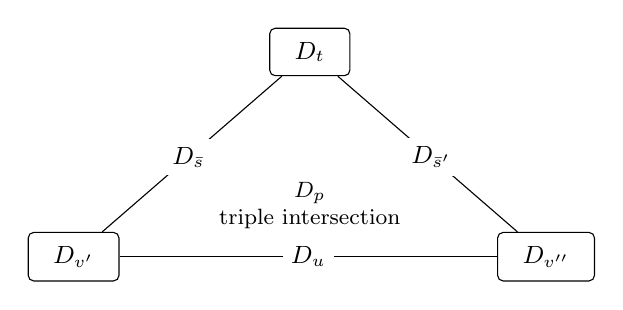
\begin{tikzpicture}[font=\small,
    diagramrange/.style={draw,rounded corners=2pt,fill=white,
                  inner xsep=9pt,inner ysep=5pt},
    overlap/.style={fill=white,inner sep=3pt}]
  \node[diagramrange] (t) at (0,1.8) {$D_t$};
  \node[diagramrange] (v) at (-3,-.8) {$D_{v'}$};
  \node[diagramrange] (w) at (3,-.8) {$D_{v''}$};
  \draw (t) -- node[overlap,pos=.52] {$D_{\bar s}$} (v);
  \draw (t) -- node[overlap,pos=.52] {$D_{\bar s'}$} (w);
  \draw (v) -- node[overlap] {$D_u$} (w);
  \node[align=center,font=\footnotesize] at (0,-.15)
    {$D_p$\\triple intersection};
\end{tikzpicture}
\caption{The independent-copy case of support descent. Each edge is
labelled by the exact intersection of its endpoint ranges. The two
placed equality witnesses $v',v''$ use the same fresh copy $u$ of $s_1$;
$t$ carries the proposed inequality between the copies on
$\bar s$ and $\bar s'$, whose ranges meet exactly in $D_p$.
These exact intersections allow the three diagrams to be amalgamated
over their common root $p$.}
\label{fig:support-descent}
\end{figure}

Every intersection in this display is its indicated common
subdiagram.  The required partial maps agree on the root, and
their domain and range sizes are at most \(\mu\);
Lemma~\ref{lem:diagram-amalgamation} therefore supplies the
ground permutations realizing these placements.

The two placed copies of \(d\) agree on \(D_u\).
They agree with \(c\) on \(D_{\bar s}\) and \(D_{\bar s'}\),
respectively, because \(c\) extends the two placed copies of
\(\delta\).  On the remaining coordinates freshness gives
compatibility.  Thus the Cohen conditions have a common extension.
The three diagrams \(v',v'',t\) also have a common extension by
Equation~\eqref{eq:descent-three-overlaps} and finite amalgamation.
The two transported \(\sigma_1\) names are literally equal,
since the placements agree on the entire \(D_{s_1}\).
The equalities transported from \((d,v)\) therefore contradict
the inequality forced by \((c,t)\).

For two active copies with arbitrary overlap, start again with
any proposed inequality-forcing common extension \((c,t)\).
Place a third copy of \(s_0\) over \(p\), independent of \(t\)
off the root, and place its Cohen trigger compatibly with \(c\).
It has a common product extension with \((c,t)\).
The independent case just proved applies between this third copy
and each of the original ones, contradicting the inequality.
This proves coherence of all active copies, below every possible
inequality witness.

Define a mixture using all joint strengthenings:
\begin{equation}\label{eq:descent-mixture}
 \sigma=
 \left\{(\pi\eta,(c,t)):
 \begin{array}{l}
 \pi\in\Fix(D_p),\quad (\eta,(a,u))\in\sigma_0,\\
 (c,t)\leq(\pi\delta,\pi s_0),\quad
 (c,t)\leq(\pi a,\pi u)
 \end{array}\right\}.
\end{equation}
This is a set name.
Left multiplication in \(\Fix(D_p)\) permutes its entries, so it
is supported by \(D_p\).
Its member names are translates of member names of \(\sigma_0\)
and hence are \(\HS\).
In any product generic its value is the union of the values of
the active copies.  Both inclusions in this description follow
from directedness of the generic: all common strengthenings,
rather than a selected one, occur in
Equation~\eqref{eq:descent-mixture}.
When the original trigger is active, coherence makes this union
exactly the value of \(\sigma_0\).
Return now to the fixed \(F\).  Since \(\delta\in F\), the
original trigger is active in every product generic with this Cohen
factor and with \(s_0\) in its diagram filter.  It follows that
\(s_0\forces_{\mathbb P}\sigma[F]=\sigma_0[F]\).
The equality with \(\sigma_1[F]\) holds below \(v\).
Its parameters are supported by \(D_{s_1}\), so
Lemma~\ref{lem:local-decision} makes it hold already below \(s_1\).

No step imposed a rank bound.
For the subset assertion, replace the mixture by its intersection
with \(A\), using the normalization in the next paragraph.
\end{proof}

For \(r\in\mathbb P\), define the following ground set of names:
\begin{equation}\label{eq:normalized-local-names}
 \mathcal X(r)=
 \left\{\tau\subseteq
     \{\dot A_j:j\in I\}\times\mathbb Q:
       (\forall\pi\in\Fix(D_r))\ \pi\tau=\tau\right\}.
\end{equation}
Every member is \(\HS\).
If a product \(\HS\) name \(\tau\) is supported by \(J\), define
\[
 \tau\mathbin{\upharpoonright} A=
 \{(\dot A_j,u):j\in I,\ u\in\mathbb Q,\
                         u\forces_{\mathbb Q}\dot A_j\in\tau\}.
\]
The ordinary truth lemma gives value \(\tau^{F\times H}\cap A\).
Symmetry preserves the support \(J\).
In particular a name supported by \(D_r\) whose actual value is
a subset of \(A\) has the same value as some member of
\(\mathcal X(r)\).
This is a set-sized normalization, valid for an original name of
any rank.

\subsection{Coding arbitrary sets by the labels}

The next argument extracts a partial function from an orbit of a name.
The diagram condition in the function's definition ensures that equal
inputs have equal values.

\begin{proposition}\label{prop:presentation}
In \(W\), every nonempty set \(X\) is the image of a surjection
\(A\times\eta\to X\) for some ordinal \(\eta\).
No bound on the rank of \(X\) is imposed.
\end{proposition}

\begin{proof}
Let \(\sigma\) be a ground \(\HS\) name, and let \(p\) have
\(D_p\) as a support for \(\sigma\).
Form the graph name
\begin{equation}\label{eq:partial-orbit-map}
 \dot h_{\sigma,p}=
 \left\{\left(
    \operatorname{op}(\dot A_{\pi(p(1))},\pi\sigma),
                      (1_{\mathbb R},\pi p)\right):\pi\in G\right\},
\end{equation}
where \(\operatorname{op}\) denotes the canonical ordered-pair name.
This name is invariant, and all its member names are \(\HS\).

Its value is a partial function on \(A\).
Indeed, suppose two contributing pairs have equal first coordinates.
Label distinctness gives
\(\pi(p(1))=\rho(p(1))\).
There is a common extension \(r\in H\) of \(\pi p,\rho p\);
write \(\pi p=r_n\) and \(\rho p=r_m\).
The equality of centers and injectivity of \(r\) give \(n=m\).
Consequently \(\pi p=\rho p\) pointwise, so
\(\rho^{-1}\pi\in\Fix(D_p)\).
It fixes \(\sigma\), and hence \(\pi\sigma=\rho\sigma\)
literally.  The two values therefore agree.
This argument concerns names under compatible diagram conditions,
not an action on one fixed symmetric model.

The orbit construction gives invariant partial functions.  We now
form a set-indexed family of them whose ranges cover \(X\).
Choose an \(\HS\) name \(\tau\) for \(X\).
The set \(M\) of member names appearing in \(\tau\) is a ground
set of \(\HS\) names.  In \(V\), enumerate by an ordinal \(\eta\)
the set
\[
 B=\{(\sigma,p)\in M\times\mathbb P:
                         \Fix(D_p)\text{ fixes }\sigma\}.
\]
Every member name has a support of size at most \(\mu\), and
Lemma~\ref{lem:diagram-amalgamation} provides supporting diagrams.
We include all such diagrams, because one chosen diagram need not
belong to the generic filter.
The corresponding sequence of graph names
\(\dot h_{\sigma,p}\) is a ground sequence of invariant
\(\HS\) names.  Its canonical sequence name is itself invariant
and \(\HS\), so its interpretation
\(\langle h_i:i<\eta\rangle\) belongs to \(W\).

These partial functions cover \(X\).
For \(x\in X\), an active member name \(\sigma\) of \(\tau\)
has value \(x\).
The set of diagrams whose ranges contain a fixed support of
\(\sigma\) is ground dense, by
Lemma~\ref{lem:diagram-amalgamation}.
Thus some such \(p\) belongs to \(H\).
The identity entry of \(\dot h_{\sigma,p}\) maps \(A_{p(1)}\)
to \(x\).

All remaining definitions take place in \(W\).
For nonempty \(X\), fix one \(x_0\in X\), and define
\[
 h(a,i)=
 \begin{cases}
 h_i(a),&a\in\dom(h_i)\text{ and }h_i(a)\in X,\\
 x_0,&\text{otherwise}.
 \end{cases}
\]
Separation and Replacement form this function on \(A\times\eta\),
and coverage makes it surjective.
The one default element uses only nonemptiness of \(X\).
The enumeration above is over \(M\times\mathbb P\), a set
depending on the particular name \(\tau\); no restriction to
names below a fixed rank was made.
\end{proof}

\subsection{Choice for ordinal-indexed families}

The presentation just proved reduces arbitrary families to families of
subsets of $A$. We first find one wellorderable part of $A$ meeting every
member of a given ordinal-indexed family of nonempty subsets.

\begin{proposition}\label{prop:ordinal-choice}
The model \(W\) satisfies \(\ACwo\): every ordinal-indexed
family of nonempty sets in \(W\) has a choice function in \(W\).
\end{proposition}

\begin{proof}
We first treat a family
\(\langle X_\xi:\xi<\eta\rangle\) of nonempty subsets of \(A\).
Start below a product condition \((d_0,p)\) forcing this
assertion for an \(\HS\) family name.
By extending the diagram, arrange that \(D_p\) contains its
support and \(\supp_I(d_0)\).
The assertions that a given graph is a function and has nonempty
subset values are absolute between \(W\) and the full extension.
Consequently this use of ordinary forcing follows equally from
a symmetric-forcing hypothesis.
Names for the individual \(X_\xi\) can be obtained by the
membership forcing relation from the family and \(\check\xi\);
they retain support \(D_p\).
Choose once and for all \(q\) with \(q_e=p\).
This same \(q\) will work for every family index.  Witnesses already
available on \(p\) need no move; for witnesses on proper extensions
of \(p\), the probes place independent copies inside \(q\) and
Cohen genericity activates one of them.

Fix \(F\) containing \(d_0\), and fix \(\xi<\eta\).
In \(V[F]\), some \(t\leq p\) and \(j\in I\) satisfy
\[
 t\forces_{\mathbb P} A_j\in X_\xi.
\]
This follows by deciding a witness in the ground index set \(I\)
for membership in \(A\).
Extend \(t\) to include \(j\) in its range, and write \(p=t_b\).
Choose \(d\in F\) witnessing the displayed forcing assertion,
and restrict it to \(D_t\) by
Lemma~\ref{lem:local-decision}.
If \(b=1\), then \(t=p\), so \(q\) already forces a witness
whose index belongs to \(D_q\).

Suppose \(b\neq1\).
The probes of Theorem~\ref{thm:monoid}, with \(a=1,U=\{1\}\),
give \(\mu\) elements \(m\) satisfying \(mb=e\) and
\(mT\cap m'T=eT\) for distinct probes.
Thus
\[
 (q_m)_b=p,\qquad
 D_{q_m}\cap D_{q_{m'}}=D_p\quad(m\neq m').
\]
Each \(q_m\) is a copy of \(t\) over \(p\).
Choose in \(V\) a permutation \(\pi_m\in\Fix(D_p)\) taking
\(t\) to \(q_m\).
The conditions \(\pi_m d\) all restrict on \(D_p\) to
\(d_*=d\restriction D_p\), and their coordinate supports off
that root are pairwise disjoint.

For these fixed ground data, the set
\begin{equation}\label{eq:probe-cohen-dense}
 \{c:c\perp d_*\}\ \cup\
 \{c:(\exists m)\ c\leq\pi_m d\}
\end{equation}
is dense in \(\mathbb R\).
Given \(c\) compatible with \(d_*\), first extend it by \(d_*\).
Its support is countable, so it meets the nonroot support of
only countably many of the pairwise disjoint copies.
Choose a remaining probe and extend \(c\) by its placed
condition \(\pi_m d\).
This proves density.
Because \(d_*\in F\), the generic meets the second alternative
of Equation~\eqref{eq:probe-cohen-dense}.
For the resulting \(m\), product symmetry and
\(\pi_m X_\xi=X_\xi\) give
\[
 q_m\forces_{\mathbb P} A_{\pi_mj}\in X_\xi
 \quad\text{in }V[F].
\]
Since \(q\leq q_m\) and \(\pi_mj\in D_q\), this supplies the
required witness in \(A[D_q]=\{A_j:j\in D_q\}\).

The condition \(q\) was chosen before \(\xi\).
Although \(t,d,j\) were chosen in the argument after \(F\),
each is an individual ground object.
The dense set in Equation~\eqref{eq:probe-cohen-dense} therefore
belongs to \(V\), and \(F\) meets it.
No sequence of witnesses for all \(\xi\) is being selected or
imported into \(W\).
For each \(\xi<\eta\) the argument shows that \(q\) forces
\(X_\xi\cap A[D_q]\neq\varnothing\) in \(V[F]\).
It forces the universal statement as well: a condition forcing
a counterexample could be strengthened to decide its index in
\(\check\eta\) to one ground \(\xi\), contradicting the
assertion for that index.
Since this holds for every \(F\) containing \(d_0\), the product
condition \((d_0,q)\) forces the universal meeting property.

A ground enumeration of \(D_q\) yields a sequence of its labels
with an \(\HS\) name supported by \(D_q\).
Distinctness of labels turns that enumeration into a wellordering
of \(A[D_q]\) in \(W\).
Taking the first element of each \(X_\xi\) in this wellordering
defines the required choice function by Replacement in \(W\).
The argument works below an extension of every starting
condition forcing the subset-family hypothesis, and hence proves
choice for all such families in \(W\).

Finally let \(\langle Y_\xi:\xi<\eta\rangle\) be any family
of nonempty sets in \(W\).
For \(\eta=0\) use the empty function.
Otherwise Proposition~\ref{prop:presentation}, applied once to
the union of the family, gives a surjection
\(h:A\times\theta\to\bigcup_{\xi<\eta}Y_\xi\) in \(W\).
For each \(\xi\), take the least \(\alpha_\xi<\theta\)
whose slice meets \(Y_\xi\), and form
\[
 B_\xi=\{a\in A:h(a,\alpha_\xi)\in Y_\xi\}.
\]
These are a family of nonempty subsets of \(A\) in \(W\).
The subset case chooses \(a_\xi\in B_\xi\);
then \(h(a_\xi,\alpha_\xi)\) is the desired choice from \(Y_\xi\).
\end{proof}

\subsection{Failure of Choice and countable-sequence preservation}

\begin{proposition}\label{prop:not-choice}
The set \(A\) is not wellorderable in \(W\).
In particular \(W\models\neg\AC\).
\end{proposition}

\begin{proof}
Suppose an \(\HS\) name is forced to be a function from an
ordinal \(\eta\) onto \(A\).
Choose a forcing condition \((d,p)\) whose diagram range contains
the name's support and \(\supp_I(d)\).
Fix \(j\notin D_p\), which exists since
\(|D_p|^V=\mu<|I|^V\).
Strengthen to a product condition \((c,t)\) deciding
a ground \(\beta<\eta\) with value \(A_j\), and extend the
diagram further to have \(j\in D_t\).

Choose \(\pi\in\Fix(D_p)\) moving all coordinates of \(t,c\)
outside \(D_p\) to fresh ones.
Then \(t,\pi t\) are independent over \(p\) and have a common
extension; \(c,\pi c\) are also compatible.
The function name and \(\check\beta\) are fixed.
Their common product extension would therefore force that
one entry has both values \(A_j\) and \(A_{\pi j}\).
They are distinct because \(j\notin D_p\) and \(\pi\) moved it
freshly.  This is a contradiction.

\end{proof}

\begin{proposition}\label{prop:no-countable-sequences}
For every ground set \(X\), every function \(f:\omega\to X\)
belonging to \(W\) belongs to \(V\).
Consequently \(W\) adds no countable sequences of ground elements.
\end{proposition}

\begin{proof}
Choose a product \(\HS\) name \(\tau\) for \(f\).
In \(V[F]\), the ordinary \(\mathbb P\)-truth lemma supplies
a condition in \(H\) forcing that \(\tau[F]\) is a function
\(\check\omega\to\check X\).
Extend within \(H\) to a diagram \(p\) whose range covers a
support of \(\tau\).
For each \(n<\omega\), the ordinary forcing theorem supplies
an extension of \(p\) and some \(x\in X\) forcing
\(\tau[F](n)=\check x\).
Both \(\tau\) and the check-name parameters are supported by
\(D_p\), so Lemma~\ref{lem:local-decision} makes \(p\)
itself force that equality.
There is exactly one such \(x\), since \(p\) forces
functionhood.

The forcing relation is definable in \(V[F]\).
Replacement there therefore forms the sequence of these unique
values, a function \(g:\omega\to X\) in \(V[F]\).
Then \(g=f\) in \(V[F][H]\), because \(p\in H\).
By Lemma~\ref{lem:cohen-properties}, \(\mathbb R\) adds no
countable sequences in the ground set \(X\), so \(g\in V\).
Thus \(f\in V\).
The final assertion follows by bounding the ranks of the entries
of any countable sequence of ground elements, as in the proof of
Lemma~\ref{lem:cohen-properties}.
\end{proof}

We have obtained the all-rank presentation and internal ordinal choice
needed for the final reduction to \(\PP\), while the labels already
witness failure of full Choice.  What remains is the quotient
classification: nonwellorderable images of \(A\) must be put in
bijection with \(A\) by one coherent, hereditarily symmetric graph.

\section{Exact fibers of a symbolic quotient}\label{sec:quotient-fibers}\label{sec:quotients}

Our next objective is a bijection between $A$ and each of its
nonwellorderable quotients. A local count of names is insufficient:
assignments made in two diagrams must agree whenever those diagrams
occur in one generic filter. We first classify local elements by the
subdiagrams on which they are available. We then construct bijections
which respect every restriction and every change of coordinates.

Throughout the quotient construction, the cardinal parameters are those
of Section~\ref{sec:forcing}, with the monoid $T$ supplied there by
Theorem~\ref{thm:monoid}. The forcing $\mathbb P$ remains the
ground set of diagrams, including when it is used after forcing with
$\mathbb R$. We use countable closure of $\mathbb R$, regularity of
$\kappa=\omega_1$, preservation of the ground cardinals $\mu,\mu^+$,
and the ground equality $\mu^{\aleph_0}=\mu$. Preservation of smaller
cardinals is unnecessary. In particular, $\mu$ always denotes the
chosen ground ordinal, not a cardinal recomputed from a new continuum.
All ground selections below are choices over specified sets in $V$.

Fix a hereditarily symmetric name $\dot E$ and a product condition
$(d_0,p)$ symmetrically forcing that $\dot E$ is an equivalence relation
on $A$ whose quotient is not wellorderable. Enlarge the diagram so that
$D_p$ supports $\dot E$ and contains $\supp_I(d_0)$. Choose $q$ with
$q_e=p$. Our bijection will have support $D_q$ and will be forced below
$(d_0,q)$. Write $G_q=\Fix(D_q)$. This group fixes $q,p,d_0$ and
$\dot E$ literally.

We write $F$ for an $\mathbb R$-generic filter containing $d_0$, and
work temporarily in $V[F]$. A product name $\tau$ determines an ordinary
$\mathbb P$-name $\tau[F]$ there. Thus an assertion such as
$r\forces\tau=\sigma$ in this section means ordinary $\mathbb P$-forcing
in $V[F]$, using these sections of the product names. The generic
notation abbreviates forcing arguments uniform below $d_0$; no claim
that a ground permutation acts on one fixed evaluated universe is used.

\subsection{Local names and their cardinal bound}

Recall the local name collection from
Equation~\eqref{eq:normalized-local-names}. A normalized subset name
means a subset of the ground set
\[
 \{(\dot A_j,(d,s)):j\in I,
                 \ (d,s)\in\mathbb R\times\mathbb P\}.
\]
For a diagram $r$, $\mathcal X(r)$ is the ground set of all such
names fixed literally by $\Fix(D_r)$. Each is hereditarily symmetric,
since its member names are the individual label names. Normalization by
the forcing relation retains any given support. When $r\le q$, define
in $V[F]$
\[
 \mathcal D_F(r)=
 \{\tau\in\mathcal X(r):
       r\forces\tau\text{ is an }\dot E\text{-class}\}/\mathord\sim_r,
 \qquad
 \tau\sim_r\sigma\ \Longleftrightarrow\ r\forces\tau=\sigma.
\]
These are quotients of ground sets, so they are sets. We sometimes omit
$F$ from the notation. Their elements are symbolic classes of names,
not yet the evaluated members of $A/E$ in a product extension.
Lemma~\ref{lem:local-decision} applies to the
class and equality tests. Consequently, for $r\le s\le q$, retaining
the same name defines an injection
\begin{equation}\label{eq:symbolic-inclusion}
 \iota_{s,r}:\mathcal D_F(s)\longrightarrow\mathcal D_F(r).
\end{equation}
Indeed, if a stronger diagram forced two local names equal, the decision
at $s$ would already be equality. These maps compose literally on
representatives. Every $j\in D_r$ has a normalized name, supported by
$D_r$, for its $E$-class: use the forcing relation to name the labels
$E$-related to $\dot A_j$. Below the present hypothesis it is an
eligible member of $\mathcal D_F(r)$.

\begin{lemma}[Local quotient bound]\label{lem:local-quotient-bound}
For every $F$ as above and every ground $r\le q$,
$|\mathcal D_F(r)|\le\mu$ in $V[F]$.
\end{lemma}
\begin{proof}
For an element choose a representative $\tau$ and a diagram $t\le r$
forcing $\tau=[\dot A_j]_E$ for some $j\in D_t$. The ordinary forcing
theorem permits deciding a representative label; extending the diagram
includes its index. Write $r=t_b$. By Cohen restriction in
Lemma~\ref{lem:local-decision}, there is $d\in F$, supported in $D_t$,
witnessing this $\mathbb P$-forcing assertion. Record the triple
\[
 (b,x,t^{-1}d),\qquad t(x)=j,
\]
where $t^{-1}d$ is the partial binary function on $T\times\kappa$
obtained by replacing each coordinate $t(y)$ with $y$. Its domain has
size less than $\kappa$. The ground set of possible records has size
at most $\mu$, since $|T|=\mu$, $\kappa\le\mu$, and
$\mu^{<\kappa}=\mu$. Its ground enumeration remains an enumeration in
$V[F]$.

Suppose two chosen representatives $\tau_1,\tau_2$ have the same
record, witnessed by $t_1,t_2,d_1,d_2,j_1,j_2$. The ground bijection
$t_1(y)\mapsto t_2(y)$ agrees with the identity on $D_r$: in both
diagrams $r=(t_i)_b$. It maps points outside $D_r$ to points outside
$D_r$. Extend it to a ground permutation $\pi$ of $I$ fixing $D_r$.
This is possible since the two ranges have size $\mu<|I|$ and their
complements have the same cardinality $|I|$. Then
\[
 \pi t_1=t_2,\qquad \pi d_1=d_2,\qquad \pi j_1=j_2,
 \qquad \pi\tau_1=\tau_1.
\]
Product symmetry makes $d_2$ witness at $t_2$ equality of both
$\tau_1$ and $\tau_2$ with $[\dot A_{j_2}]_E$. Since $d_2\in F$,
$t_2$ forces $\tau_1=\tau_2$ in $V[F]$. Decision at $r$ gives the
same equality there. Thus distinct elements have distinct records.
Choosing representatives and records uses Choice in the ordinary
extension $V[F]$, not in the symmetric model.
\end{proof}

\subsection{Availability and exact multiplicities}

For $r\le q$, write $q=r_a$. For $h\in\mathcal D_F(r)$ and
$j\in D_r$, respectively, define
\begin{align}
 U_h&=\{n\sqsubseteq a:
             h\in\ran(\iota_{r_n,r})\},\label{eq:class-availability}\\
 U_j&=\{n\sqsubseteq a:j\in D_{r_n}\}.
             \label{eq:label-availability}
\end{align}
An ideal here is nonempty, downward closed, and closed under finite
joins. All joins needed within $\downarrow a$ exist.

\begin{lemma}[Availability ideals]\label{lem:availability-ideals}
Each set in Equations~\eqref{eq:class-availability} and
\eqref{eq:label-availability} is an ideal of $\downarrow a$.
Every ideal of $\downarrow a$ in $V[F]$ belongs to $V$.
\end{lemma}
\begin{proof}
Both sets contain $1$ and are downward closed by inclusion of
subdiagrams. Suppose $n,n'\in U_h$ and put $k=n\vee n'$. The ranges
of $r_n,r_{n'}$ intersect exactly in $D_{r_k}$. Choose supported names
for their representations of $h$. They are forced equal by $r$.
Lemma~\ref{lem:support-descent}, with root $r_k$, supplies a
$D_{r_k}$-supported name equal to them. Normalize it without changing
support. Decision at $r_k$ shows it is an $E$-class there: its
negation would persist to the extension $r$. Thus $k\in U_h$.
For labels the identical argument is the literal equality of cone
intersections, without any name descent.

For the final assertion, apply Lemma~\ref{lem:mono-countable-ideal}
in $V[F]$. The ground monoid, order, heights and costs retain their
meanings there, so every nonempty ideal has a countable cofinal sequence.
It consists of ground elements of $T$, so countable closure of
$\mathbb R$ puts it in $V$. Its downward closure, computed with the
unchanged ground order, is the original ideal. The argument applies
to every ideal in $V[F]$, not only to ground ideals.
\end{proof}

For a nonempty ideal $U\subseteq\downarrow a$, put
\[
 B_{r,U}(F)=\{h\in\mathcal D_F(r):U_h=U\},\qquad
 L_{r,U}=\{j\in D_r:U_j=U\}.
\]
The second set is ground data; the first can depend on $F$.
These exact fibers, rather than the whole local sets $\mathcal D_F(r)$,
are the pieces on which a bijection can respect restriction: a label
and its assigned class must remain available at precisely the same
subdiagrams.

\begin{lemma}[Exact fibers]\label{lem:exact-fibers}
For every $r\le q$ and every nonempty ideal
$U\subseteq\downarrow a$, where $q=r_a$, both $B_{r,U}(F)$ and
$L_{r,U}$ have cardinality $\mu$ in $V[F]$. The label fiber already
has that cardinality in $V$.
\end{lemma}
\begin{proof}
The common root $p$ will separate the copies used in this proof.
We first find a class with no representation supported by $D_p$.
Copying it into diagrams whose unwanted intersections are exactly
$D_p$ will then rule out both coincidences between copies and
availability at forbidden subdiagrams, by support descent.

\smallskip\noindent\textit{A class unavailable at the root.}
Enumerate
$\mathcal X(p)$ in $V$ as $(\tau_\xi:\xi<\lambda)$. The canonical
name for the sequence of its evaluations is hereditarily symmetric
with support $D_p$. Explicitly, its entries are the canonical pairs
$(\check\xi,\tau_\xi)$, each placed under every product condition.
Every member of $\Fix(D_p)$ fixes each entry literally. The range
of this sequence is wellorderable inside $W$: map each value to its
least index of occurrence. If it contained every $E$-class, the same
map restricted to $A/E$ would wellorder that quotient. The hypothesis
therefore implies, ordinarily below $(d_0,p)$, that some $E$-class
lies outside the evaluations of all names in $\mathcal X(p)$.

Fix $F$ containing $d_0$. By the ordinary forcing theorem choose
$t\le p$ and $j\in D_t$ such that $t$ forces the class of $A_j$
outside that entire evaluation list. Choose a witnessing Cohen
condition $d\in F$ supported in $D_t$, using
Lemma~\ref{lem:local-decision}. Write $p=t_b$. Necessarily $b\ne1$,
since a class represented by a label in $D_p$ has a name in
$\mathcal X(p)$.

\smallskip\noindent\textit{Independent copies with active Cohen conditions.}
As $p=r_{ae}$, the probe property of Theorem~\ref{thm:monoid}
supplies $\mu$ elements $m$ with $mb=ae$ and the prescribed ideal
$U$. The diagrams $r_m$ are copies of $t$ over $p$, with pairwise
intersection exactly $D_p$. Choose the ground permutations taking
$t$ to these diagrams and fixing $D_p$, and transport $d$ and the
class name along them. Their nonroot coordinate sets are disjoint.
This is the role of the earlier extension $q_e=p$: the availability
pattern is prescribed among divisors of $a$, while the common root
lies at $ae$, strictly beyond $a$.

There are $\mu$ copies whose transported Cohen conditions belong to
$F$. To see this without any $\mu$-closure assertion, partition the
ground family into $\mu$ ground subfamilies of size $\mu$. In each
subfamily the conditions extending at least one transported copy of
$d$ form a dense set below $d\restriction D_p$. Indeed, a Cohen
condition uses countably many coordinate indices; among the pairwise
disjoint nonroot ranges there is one it misses, and on the root the
two conditions agree. Their union is a Cohen condition. Genericity
meets each of these ground dense sets. A hit in each disjoint
subfamily yields $\mu$ different hits.

\smallskip\noindent\textit{Distinct classes with the prescribed exact ideal.}
Each hit gives a $D_{r_m}$-supported class name forced at $r_m$
to lie outside the evaluations of $\mathcal X(p)$. The diagram
$r_m$ extends $p$ but need not extend $q$; we use its class name,
not a set $\mathcal D_F(r_m)$. As $r$ extends $r_m$, this name
represents a symbolic class in the defined set $\mathcal D_F(r)$.
Two such
classes cannot be equal there: support descent over their common
root $p$ would supply a name in $\mathcal X(p)$ for their common
value, contrary to the outside assertion. If $n\in U$, then
$n\sqsubseteq m$, so $r_n$ extends $r_m$ and the class is available
at $r_n$. If $n\sqsubseteq a$ and $n\notin U$, the exact probe
intersection gives
\[
 nT\cap mT=aeT,
 \qquad D_{r_n}\cap D_{r_m}=D_p.
\]
Availability at $r_n$ would again descend to a name in
$\mathcal X(p)$, a contradiction. Its exact availability ideal is
therefore $U$. This gives $\mu$ distinct elements of $B_{r,U}(F)$;
Lemma~\ref{lem:local-quotient-bound} bounds that fiber from above.

\smallskip\noindent\textit{The label fiber.}
For labels use the probe centers $r(m)$. Their availability ideals
are exactly $\downarrow m\cap\downarrow a=U$, and distinct probes
have distinct centers. This supplies a ground $\mu$-subset of
$L_{r,U}$; the upper bound follows from $|D_r|=\mu$.
\end{proof}

\section{Components of subdiagrams and their stabilizers}
\label{sec:quotient-components}

The exact fibers have equal cardinality, but choosing their bijections
independently would not preserve assignments when a diagram is replaced
by a subdiagram. We first show that restriction identifies entire
exact fibers, not merely subsets of them. Following these canonical
identifications groups the fibers into components. Only after forming
the components will we choose bijections; their stabilizers determine
which symmetries those choices must respect.

\subsection{Contractions and canonical identifications}

A vertex is a pair $v=(r,U)$, where $r\le q$, $q=r_a$, and $U$ is a
nonempty ideal of $\downarrow a$. Vertices form a ground set by
Lemma~\ref{lem:availability-ideals}. For $n\in U$ define a
\emph{contraction}
\begin{equation}\label{eq:quotient-contraction}
 (r,U)\longrightarrow(r_n,U_n),\qquad
 U_n=\{x\sqsubseteq c:nx\in U\},\quad nc=a.
\end{equation}
Left multiplication preserves conditional joins. In fact cancellation
and the common-cone description of a join give
$n(x\vee y)=nx\vee ny$ whenever these elements have a common right
multiple. It follows that $U_n$ is an ideal. Contractions compose;
there is at most one contraction between fixed endpoints, since the
center of $r_n$ is $r(n)$ and $r$ is injective. Write $B_v(F)$ and
$L_v$ for the two fibers at a vertex.

\begin{lemma}[Contraction identifications]\label{lem:contraction-fibers}
For every contraction $v\to w$, the label fibers satisfy $L_v=L_w$,
and inclusion of symbolic elements gives a bijection
$B_w(F)\longrightarrow B_v(F)$. These identifications commute with
composition.
\end{lemma}
\begin{proof}
Let $v=(r,U)$, $w=(r_n,U_n)$, and first take a symbolic class
available at $r_n$. Its full availability ideal $J$ at $r$ contains
$n$. For $z\sqsubseteq a$, ideal closure gives
\[
 z\in J\quad\Longleftrightarrow\quad z\vee n\in J.
\]
Write $z\vee n=nx$. Availability at $r_{z\vee n}$ is exactly the
corresponding availability at the subdiagram $(r_n)_x$ of $r_n$.
Thus the restricted ideal at $r_n$ determines the full ideal at $r$.
If that restricted ideal is $U_n$, the last test is equivalent to
$z\vee n\in U$, and hence to $z\in U$. Conversely, an element of
$B_v(F)$ is available at $r_n$ because $n\in U$, and its restricted
ideal is $U_n$. This proves surjectivity; injectivity follows from
Equation~\eqref{eq:symbolic-inclusion}. For labels use the same
argument with literal membership in ranges. Commutation follows
because all the symbolic maps retain the same representative names.
\end{proof}

Let a component be a connected component of the vertex system when
the direction of contractions is ignored. The successors of each
vertex are directed: contract at the join of two contraction indices.
Any two vertices in one component have a common successor. Indeed,
this holds along a single edge; along a finite path combine a common
successor of its initial part with the final edge, using directedness
of successors at the shared vertex. The same induction gives a common
successor for any finite set of vertices in a component.

Consequently all finite chains of the identifications in
Lemma~\ref{lem:contraction-fibers} are consistent. One can compare a
finite chain at a common successor, where both composites are the
same map. In a component $C$, glue the disjoint union of its $B_v(F)$
by these identifications and call the resulting set $B_C(F)$. Each
fiber maps bijectively onto $B_C(F)$. In particular, the gluing creates
no new identifications within one fiber. All label fibers in $C$
are the same ground subset of $I$; denote it by $L_C$. Both sets have
cardinality $\mu$ in $V[F]$.

Choose in $V$ a vertex $(r,U)$ of $C$ and a nondecreasing cofinal
sequence $(n_i:i<\omega)$ in $U$, with $n_0=1$. Let $v_i$ be its
contraction at $n_i$. This chain is cofinal in the entire component.
To check this, compare any vertex with $v_0$ at a common successor,
which is a contraction of $v_0$ at some $n\in U$. Choose $i$ with
$n\sqsubseteq n_i$. Then $v_i$ is a successor of that common
successor and hence of the given vertex.

\subsection{Only countably many residual symmetries}

The group $G_q$ acts on the ground vertex system. On symbolic fibers
it acts by transport between generics:
\begin{equation}\label{eq:symbolic-transport}
 T_\pi^F:\mathcal D_F(r)\longrightarrow
                   \mathcal D_{\pi F}(\pi r),
 \qquad [\tau]_r\longmapsto[\pi\tau]_{\pi r}.
\end{equation}
The forcing symmetry lemma makes this well defined, and it commutes
with all contraction identifications. We use the same notation for
transport on the glued fibers, and suppress the superscript when its
source generic is specified by the argument.

Let $G_C$ be the setwise stabilizer of $C$ in $G_q$. Define
\[
 K_C=\bigcup_{i<\omega}\Fix(D_{r_{n_i}}).
\]
Each displayed fixer is a subgroup of $G_q$, because $D_q$ is contained
in every chain range. It fixes a vertex and therefore lies in $G_C$.
The ranges decrease, so the subgroups increase and their union is a
subgroup. For $\sigma\in G_C$, the moved chain is also cofinal.
For every $i$ there is $j$ with
$D_{r_{n_j}}\subseteq D_{\sigma r_{n_i}}$. Hence
\[
 \sigma\Fix(D_{r_{n_i}})\sigma^{-1}
 =\Fix(D_{\sigma r_{n_i}})\subseteq\Fix(D_{r_{n_j}}).
\]
Applying the same reasoning to $\sigma^{-1}$ proves that $K_C$ is
normal in $G_C$.

\begin{lemma}[Countable stabilizer quotient]\label{lem:countable-germs}
In the ground model, $|G_C/K_C|\le\aleph_0$.
\end{lemma}
\begin{proof}
Choose the countable-base tower of Theorem~\ref{thm:monoid} so that
its initial submonoid $T_0$ contains all $n_i$ and all right
quotients between them. For $\pi\in G_C$, consider its alignments
with contractions of the chosen vertex:
\[
 \mathcal A_\pi=
 \{(l,m)\in\omega\times U:\pi r_{n_l}=r_m\}.
\]
This set is nonempty: the moved chain is cofinal in $C$, so one of
its terms is a successor of $v_0$. Every second coordinate $m$ of
an alignment divides some $n_N$, by cofinality of $(n_i)$ in $U$.

To apply Lemma~\ref{lem:mono-descent}, fix $(l,m)\in\mathcal A_\pi$
and any $N$. Choose $l'\ge l$ so that $\pi v_{l'}$ is a successor
of $v_N$. Its diagram is $r_k$ for some $k\in U$ with
$n_N\sqsubseteq k$. Let $d\in T_0$ be the right quotient
$n_ld=n_{l'}$. Then
\[
 r_k=\pi r_{n_{l'}}=(\pi r_{n_l})_d=r_{md}.
\]
Injectivity of $r$ gives $k=md$. Consequently $md\in U$,
$n_N\sqsubseteq md$, and $(l',md)\in\mathcal A_\pi$.
These are exactly the replacement hypotheses of
Lemma~\ref{lem:mono-descent}. Its conclusion supplies an alignment
$(l,m)$ with $m\in T_0$.

There are countably many resulting alignment pairs
$(l,m)\in\omega\times T_0$. Two permutations giving the same pair
agree pointwise on $D_{r_{n_l}}$; if they are $\pi$ and $\rho$,
then $\pi^{-1}\rho\in\Fix(D_{r_{n_l}})\subseteq K_C$.
Enumerate the pairs, and assign to each coset the first
pair realized by any of its members. Distinct cosets receive distinct
pairs. This proves the bound.
\end{proof}

\section{Equivariant assignments and the quotient bijection}
\label{sec:quotient-equivariance}

For each component $C$ we seek a bijection
$f_C(F):L_C\to B_C(F)$ satisfying
\begin{equation}\label{eq:component-covariance}
 f_C(\sigma F)(\sigma j)=T_\sigma^F(f_C(F)(j))
              \qquad(\sigma\in G_C).
\end{equation}
This is an identity between computations at different generics, not
an action on one fixed extension. We first construct a bijection
covariant under $K_C$: its elements fix a sufficiently late subdiagram,
so they fix the tails of suitable name codes. We then handle the
remaining countable quotient $G_C/K_C$. Bounded Cohen-row patterns
distinguish its cosets and select a transported bijection with the
full covariance in Equation~\eqref{eq:component-covariance}.

\subsection{An assignment invariant under a tail fixer}

For the chosen chain of $C$, let $\mathcal Q_C$ be the ground set of
sequences
\[
 c=(\tau_i:i<\omega),\qquad \tau_i\in\mathcal X(r_{n_i}).
\]
Say that $c$ represents $b\in B_C(F)$ if, from some index onward,
$\tau_i$ represents an element of the exact fiber $B_{v_i}(F)$ and
its image in $B_C(F)$ is $b$. Finite initial segments are ignored.
Every $b$ has such a code: choose representatives at all chain
vertices in $V[F]$, using their bijections with $B_C(F)$. This is a
countable sequence of ground name codes, and hence belongs to $V$
by countable closure of $\mathbb R$.

Fix a ground wellordering of $\mathcal Q_C$, of order type $\lambda_C$.
Assign to $b$ its least representing code. Distinct $b$ have different
codes, so this defines a wellorder $<_F$ of $B_C(F)$.

\begin{lemma}[Covariance of the least-code order]
\label{lem:least-code-covariance}
For every $k\in K_C$, transport $T_k^F$ is an order isomorphism
from $(B_C(F),<_F)$ to $(B_C(kF),<_{kF})$. The group $K_C$ fixes
$L_C$ pointwise.
\end{lemma}
\begin{proof}
Choose $N$ such that $k$ fixes $D_{r_{n_N}}$ pointwise. For $i\ge N$
it fixes $r_{n_i}$ and every name in $\mathcal X(r_{n_i})$ literally.
Consequently each particular ground code $c$ represents $b$ at $F$
if and only if the \emph{same code} represents $T_k^F(b)$ at $kF$.
The forcing symmetry lemma proves this on the tail; the definition
ignores the remaining finite prefix. Thus the sets of functioning
codes are identical, and their minima under the fixed ground
wellorder are identical. This proves the order assertion. Also
$L_C\subseteq D_{r_{n_i}}$ for every $i$, so $k$ fixes its every
member.
\end{proof}

Let $\theta_C(F)$ be the order type of this order. It is at most
$\lambda_C$, since it is the order induced on a subset of the ordered
code set. It has cardinality $\mu$ in $V[F]$. Preservation of $\mu$
and $\mu^+$ implies
\[
 \mu\le\theta_C(F)<\mu^+,
 \qquad |\theta_C(F)|^V=\mu.
\]
Here the order type is an ordinal, hence a ground ordinal. The two
preserved cardinal endpoints justify the last equality even if smaller
cardinals have collapsed. In $V$, choose bijections
$e_\theta:\mu\longrightarrow\theta$ for the set of ordinals
$\theta\le\lambda_C$ with ground cardinality $\mu$. Also fix a ground
bijection $l_C:\mu\longrightarrow L_C$. If
$b_F:\theta_C(F)\longrightarrow B_C(F)$ is the unique order
isomorphism, define
\[
 f_C^0(F)=b_F\circ e_{\theta_C(F)}\circ l_C^{-1}.
\]
This is a bijection $L_C\to B_C(F)$. All choices have been restricted
to sets; no simultaneous choice over a proper class of ordinals occurs.
Lemma~\ref{lem:least-code-covariance} gives
\begin{equation}\label{eq:preliminary-covariance}
 f_C^0(kF)(j)=T_k^F\bigl(f_C^0(F)(j)\bigr)
       \qquad(k\in K_C,\ j\in L_C).
\end{equation}
The ground wellorder of all codes need not be invariant under $k$.
The proof uses eventual fixation of each code's entries instead.

\subsection{Detecting and choosing a coset}

Put $\Gamma_C=G_C/K_C$, writing cosets as $\pi K_C$. It is a
countable ground
group by Lemma~\ref{lem:countable-germs}. For each nonidentity coset
$\delta$, choose a ground representative $\gamma_\delta$ and points
\[
 s_{\delta,i}\in D_{r_{n_i}},\qquad
 \gamma_\delta(s_{\delta,i})\ne s_{\delta,i}
       \quad(i<\omega).
\]
Such a point exists for every $i$, since otherwise
$\gamma_\delta\in K_C$. Fix an enumeration of the set of nonidentity
cosets. For $\alpha<\kappa$ and $\pi\in G_C$, define the pattern
\begin{equation}\label{eq:detector-pattern}
 P_F^\alpha(\pi K_C)=
 \left(
  \left[\left(A_{\pi(s_{\delta,i})}^F
                       \restriction\alpha:i<\omega\right)\right]_{\rm ev}
              :\delta\in\Gamma_C\setminus\{1\}\right),
\end{equation}
where $[\cdot]_{\rm ev}$ denotes equivalence modulo eventual equality
of sequences. We regard each row as its binary characteristic
function. The equivalence classes in this formula are taken in the
ground set of sequences of subsets of $\alpha$.

This ground interpretation is legitimate. Every $\alpha<\omega_1$
is countable. The bounded row restrictions and all their countably
many coordinates, for all detectors, form a countable sequence of
ground bits and indices. Since $\mathbb R$ adds no such sequences,
these data belong to $V$. Eventual equality between ground sequences
has the same meaning in the extension. For all $\alpha<\kappa$
together the possible patterns form a ground set, on which choose a
ground wellorder, separately for each $\alpha$ if desired.

\begin{lemma}[A covariant coset selector]\label{lem:coset-selector}
Formula~\eqref{eq:detector-pattern} is independent of the
representative of $\pi K_C$. For each $F$ there is an
$\alpha<\kappa$ at which all distinct cosets have distinct patterns.
There is a definable selection $c_C(F)\in\Gamma_C$ satisfying
\begin{equation}\label{eq:coset-selector-covariance}
 c_C(\sigma F)=\sigma c_C(F)\qquad(\sigma\in G_C).
\end{equation}
\end{lemma}
\begin{proof}
If $k\in K_C$, it fixes all $s_{\delta,i}$ once $i$ is sufficiently
large. Replacing $\pi$ with $\pi k$ therefore changes each detector
sequence in only finitely many places, proving representative
independence.

Suppose $\pi K_C\ne\pi'K_C$. Use the detector for
$\delta=(\pi^{-1}\pi')K_C$ and write
$\pi^{-1}\pi'=\gamma_\delta k$ with $k\in K_C$. Eventually
$k(s_{\delta,i})=s_{\delta,i}$, and hence
\[
 \pi(s_{\delta,i})\ne\pi'(s_{\delta,i}).
\]
Distinct label indices give distinct Cohen rows. For each of these
tail positions choose a bit where the two rows differ. The countably
many bit ordinals are bounded below regular $\kappa$. Above that
bound the two restricted sequences disagree at every position on a
tail, so are unequal modulo eventual equality. There are countably
many pairs of cosets; a further countable supremum supplies one bound
that distinguishes all pairs. These choices take place in $V[F]$.
They use regularity of $\kappa$, not closure of $\mathbb P$.

At the least distinguishing $\alpha$, choose the coset whose pattern
is least in the fixed ground wellorder. If $\Gamma_C$ is trivial,
choose its sole element and use $\alpha=0$. For $\sigma\in G_C$,
label transport gives, for every $s\in I$,
$A_{\sigma s}^{\sigma F}=A_s^F$. Thus
\begin{equation}\label{eq:pattern-covariance}
 P_{\sigma F}^\alpha((\sigma\pi)K_C)
                    =P_F^\alpha(\pi K_C).
\end{equation}
The actual ground pattern objects on the two sides are equal. Left
multiplication permutes the coset set, so the least distinguishing
bound is unchanged and the same pattern object is minimal. This
proves Equation~\eqref{eq:coset-selector-covariance}.
\end{proof}

For a coset $\gamma=\pi K_C$, define a transported preliminary
bijection by
\begin{equation}\label{eq:coset-assignment}
 f_C^\gamma(F)(j)=
 T_\pi^{\pi^{-1}F}
       \left(f_C^0(\pi^{-1}F)(\pi^{-1}j)\right),\qquad j\in L_C.
\end{equation}
Equivalently, the square in Figure~\ref{fig:moved-generic-transport}
commutes.

\begin{figure}[htbp]
\centering
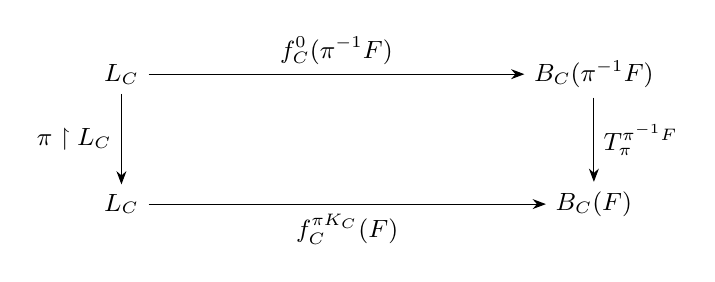
\begin{tikzpicture}[font=\small,>=Stealth]
  \node (a) at (0,1.65) {$L_C$};
  \node (b) at (6,1.65) {$B_C(\pi^{-1}F)$};
  \node (c) at (0,0) {$L_C$};
  \node (d) at (6,0) {$B_C(F)$};
  \draw[->] (a) -- node[above] {$f_C^0(\pi^{-1}F)$} (b);
  \draw[->] (a) -- node[left] {$\pi\restriction L_C$} (c);
  \draw[->] (b) -- node[right] {$T_\pi^{\pi^{-1}F}$} (d);
  \draw[->] (c) -- node[below] {$f_C^{\pi K_C}(F)$} (d);
\end{tikzpicture}
\caption{Transporting a preliminary bijection, for $\pi\in G_C$.
The square commutes: to assign the bottom label $j$, first compute
at $\pi^{-1}j$ in the generic $\pi^{-1}F$, then transport the result
to $F$. The top and bottom computations use $\pi^{-1}F$ and $F$,
respectively.}
\label{fig:moved-generic-transport}
\end{figure}


This is independent of $\pi$. Replacing $\pi$ with $\pi k$ inserts
$k^{-1}$ in the source generic, and
Equation~\eqref{eq:preliminary-covariance} cancels its transport;
$k$ fixes every label of $L_C$. Define
$f_C(F)=f_C^{c_C(F)}(F)$. Equations~\eqref{eq:coset-selector-covariance}
and~\eqref{eq:coset-assignment} now give the required
Equation~\eqref{eq:component-covariance}.
This calculation explains why the preliminary computation in
Equation~\eqref{eq:coset-assignment} is made at $\pi^{-1}F$.
An arbitrary transport of the computation at $F$ would not give the
required identity.

\subsection{Transport over all components}

Choose in $V$ one representative from each $G_q$-orbit of components
and perform the preceding set-sized choices for these representatives.
For $C'=\sigma C$, transport $f_C(\sigma^{-1}F)$ by $\sigma$ to
obtain $f_{C'}(F)$. Two possible choices of $\sigma$ differ by an
element of $G_C$, so Equation~\eqref{eq:component-covariance} proves
that this definition is independent of the choice. It yields
bijections for every component, covariant under all $G_q$. Pulling
back along the canonical maps $B_v(F)\to B_C(F)$ gives bijections
\begin{equation}\label{eq:coherent-fiber-bijections}
 f_{r,U}(F):L_{r,U}\longrightarrow B_{r,U}(F).
\end{equation}
They commute with every contraction, and their transports under every
$\pi\in G_q$ are the corresponding bijections at $\pi F$.

We record the definability needed to convert these computations into
one symmetric name. The ground sets of vertices, components, name
codes, code wellorders, patterns and auxiliary bijections are all
sets. The sections of the product names can be constructed in an
$\mathbb R$-extension from its generic filter; the ordinary forcing
relation for the ground set poset $\mathbb P$ is definable there.
Symbolic quotients and their gluing use equivalence relations on sets.
All remaining steps use set operations, least elements of prescribed
wellorders, and unique order isomorphisms. They therefore define,
by an ordinary set-theoretic formula in an $\mathbb R$-extension, the
predicate
\begin{equation}\label{eq:assignment-predicate}
 \Phi(F,r,j,\tau):
 \quad \tau\in\mathcal X(r)\text{ represents }
 f_{r,U_j}(F)(j)\text{ in }\mathcal D_F(r).
\end{equation}
Here $U_j$ is ground data from Equation~\eqref{eq:label-availability}.
One formal implementation uses a ground set of all normalized name
codes and its ordinary name-evaluation relation to construct their
$\mathbb P$-sections. The variable for a ground code and the actual
forcing name that it codes are kept distinct. In particular, we never
use the false assertion that an automorphism moves a check-name for a
ground code to the check-name for its transported code.

The proved semantic covariance is the identity
\[
 \Phi(F,r,j,\tau)\quad\Longleftrightarrow\quad
 \Phi(\pi F,\pi r,\pi j,\pi\tau)
       \qquad(\pi\in G_q).
\]
These computations are ordinary forcing arguments for this fixed
formula. More explicitly, let
\[
 \dot F^{\pi}=
 \{(\check{\pi d},d):d\in\mathbb R\},
\]
whose value at $F$ is $\pi F$. The preceding covariance proof gives
the equivalence, forced by $d_0$ in $\mathbb R$, between
$\Phi(\dot F,r,j,\tau)$ and
$\Phi(\dot F^{\pi},\pi r,\pi j,\pi\tau)$, with all auxiliary
ground choices fixed. Under the name action,
$\pi\dot F^{\pi}=\dot F$ literally, while check names for the
displayed ground arguments remain fixed. Applying ordinary forcing
symmetry therefore gives
\begin{equation}\label{eq:assignment-forcing-covariance}
 d\forces_{\mathbb R}\Phi(\dot F,r,j,\tau)
 \quad\Longleftrightarrow\quad
 \pi d\forces_{\mathbb R}
                  \Phi(\dot F,\pi r,\pi j,\pi\tau)
 \qquad(d\le d_0).
\end{equation}
All auxiliary ground choices are already fixed in the defining
formula; covariance was proved for this one construction. The
$\mathbb R$-forcing values in this display are ground sets of
conditions. Equivalently, if $F'$ contains $\pi d$, put
$F=\pi^{-1}F'$ and apply covariance to the computation at $F$;
the converse uses $\pi^{-1}$. This generic description abbreviates
the fixed-formula argument above and requires no transitive-ground
assumption in the consistency deduction.

\subsection{One hereditarily symmetric graph}

\begin{theorem}[Quotient classification]\label{thm:quotient-classification}
In $W$, every nonwellorderable surjective image of $A$ is in bijection
with $A$.
\end{theorem}
\begin{proof}
We first finish the construction for the equivalence relation fixed
at the start of Section~\ref{sec:quotient-fibers}. Use canonical
equivariant ordered-pair names and form the product name
\begin{equation}\label{eq:quotient-bijection-name}
 \dot J=
 \left\{
 \left(\langle\dot A_j,\tau\rangle^{\bullet},(d,r)\right):
 \begin{array}{l}
 r\le q,\ j\in D_r,\ \tau\in\mathcal X(r),\ d\le d_0,\\
 d\forces_{\mathbb R}\Phi(\dot F,r,j,\tau)
 \end{array}\right\}.
\end{equation}
The superscript denotes the name for the ordered pair. This is a set
name: every index ranges over a ground set and the defining forcing
relation is a ground relation. Equation~\eqref{eq:assignment-forcing-covariance}
sends each entry under $\pi\in G_q$ to another entry. Applying
$\pi^{-1}$ gives equality of the sets of entries, so $G_q$ fixes
$\dot J$ literally. Each member name is a pair of HS names; thus
$\dot J$ is HS with support $D_q$. The individual member names may
have different supports. Hereditary symmetry does not require all of
them to use $D_q$.

Take a product generic $(F,H)$ containing $(d_0,q)$. For every
$r\in H$ below $q$, the graph contains exactly the local assignments
of Equation~\eqref{eq:coherent-fiber-bijections}. In detail, whenever
$\Phi(F,r,j,\tau)$ holds, the $\mathbb R$ truth lemma gives a
condition of $F$ forcing it; strengthening with $d_0$ retains a
condition of $F$, and Equation~\eqref{eq:quotient-bijection-name}
includes its entry. Conversely, every active entry forces its
asserted assignment. All classes are represented by names in their
symbolic equivalence classes, so the local assignments are complete.

We check the comparison when the diagram is strengthened. Suppose
$t\le r\le q$, $r=t_b$, and $j\in D_r$. The availability ideal
of $j$ at $t$ contains $b$. Hence
\[
 (t,U_j\text{ computed at }t)
        \longrightarrow(r,U_j\text{ computed at }r)
\]
is a contraction. Equation~\eqref{eq:coherent-fiber-bijections}
therefore gives the same assigned symbolic element under inclusion.
In particular, its product-name evaluations are equal in every
$\mathbb P$-generic containing $t$.

Any two active entries of $\dot J$ occur together below a common
stronger diagram in $H$. At that diagram the union of the
exact-fiber bijections is a bijection
$D_t\to\mathcal D_F(t)$: availability ideals partition both sets.
The preceding comparison proves single-valuedness and injectivity of
$\dot J^{F,H}$. Distinct symbolic elements are forced unequal there
by local decision, and distinct indices have distinct Cohen labels.
Thus these are also single-valuedness and injectivity for the actual
sets of the graph.

Every label index belongs to a diagram in $H$ below $q$, by the
density of extending diagrams to contain prescribed supports.
Therefore the graph has domain $A$. To reach an arbitrary $E$-class,
take any label belonging to that class and include its index in such
a diagram $r$. Its canonical supported class name represents an
element of $\mathcal D_F(r)$. The local fiber bijection is onto the
fiber containing that element, so the graph reaches the class.
This is a pointwise existence argument; no simultaneous selection
of representatives of all classes has been made. The range is
exactly $A/E$. The graph belongs to $W$ because its name is HS.

The construction was made on an extension of an arbitrary symmetric
condition asserting the nonwellorderable-quotient hypothesis. Applying
the symmetric forcing theorem and truth lemma therefore proves in
$W$ that every such quotient $A/E$ is in bijection with $A$.
Finally, for a surjection $h:A\to Y$ in $W$, form its kernel
relation $E$ in $W$. The map $[a]_E\mapsto h(a)$ is a bijection
$A/E\to Y$, defined by its unique values without choosing class
representatives. If $Y$ is nonwellorderable, so is $A/E$, and composing
this bijection with the one just constructed proves the theorem.
\end{proof}

\section{From quotient classification to the Partition Principle}
\label{sec:conclusion}

We now pass from the classification of quotients of the label set to
arbitrary surjections.  The reduction uses only three statements inside
the symmetric model: every nonempty set is an image of the label set
times an ordinal, choice holds for ordinal-indexed families, and every
nonwellorderable image of the label set is bijective to it.  We first
prove this reduction in $\ZF$, independently of the construction.

The ordinal slicing and assembly of injections follow the local-to-global
method in Ryan-Smith's analysis of $\PP$
\cite[Propositions~3.17 and~3.20]{RyanSmith2025}. We use the stronger
classification of nonwellorderable images stated below and give the
complete reduction under these hypotheses.

\begin{lemma}[The all-set reduction]\label{lemma:pp-reduction}
Work in $\ZF$.  Suppose that a nonempty set $A$ has the following
properties.
\begin{enumerate}
\item For every nonempty set $X$, there are an ordinal $\eta$ and
a surjection $A\times\eta\longrightarrow X$.
\item Every ordinal-indexed family of nonempty sets has a choice
function.
\item Every nonwellorderable surjective image of $A$ is in bijection
with $A$.
\end{enumerate}
Then $\PP$ holds: for all sets $X,Y$, every surjection
$f:X\longrightarrow Y$ has an injection $j:Y\longrightarrow X$.
\end{lemma}

\begin{proof}
We will use two elementary observations about images of $A$.
If $h:A\longrightarrow B$ is onto and $\varnothing\ne S\subseteq B$,
then $S$ is also an image of $A$.  Indeed, fix one $s_0\in S$ and
define
\[
 h_S(a)=
 \begin{cases}
 h(a),&h(a)\in S,\\
 s_0,&h(a)\notin S.
 \end{cases}
\]
This proves an existence assertion for one given nonempty subset;
it does not choose a default element simultaneously for a family.
Also, the image of a wellorderable set under any function is
wellorderable: order its image by the least preimages in a fixed
wellordering of its domain.  Both observations are theorems of $\ZF$.

Fix a surjection $f:X\longrightarrow Y$.  If $Y=\varnothing$, the
empty function is the desired injection.  Otherwise $X$ is nonempty.
Choose a surjection $s:A\times\eta\longrightarrow X$ from the first
assumption.  Define, for $i<\eta$,
\begin{align}
 B_i&=s[A\times\{i\}],\notag\\
 Y_i&=f[B_i]\setminus\bigcup_{k<i}f[B_k],\notag\\
 S_i&=B_i\cap f^{-1}[Y_i].\label{eq:final-disjoint-slices}
\end{align}
Separation and Replacement form these sequences.  Every $y\in Y$
belongs to $f[B_i]$ for some $i$, and its least such index is the
unique index for which $y\in Y_i$.  Thus the $Y_i$ partition $Y$.
The $S_i$ are pairwise disjoint because their $f$-images lie in the
pairwise disjoint $Y_i$.  Moreover,
\[
 f\mathbin{\upharpoonright}S_i:S_i\longrightarrow Y_i
\]
is onto for every $i$.  The sets $S_i$ need not cover $X$.

Before choosing any injections, define
\begin{equation}\label{eq:final-candidate-injections}
 \begin{split}
 \mathcal J_i=\{j\in\mathcal P(Y\times X):{}&
    j\text{ is an injective function},\\
    &\dom(j)=Y_i,\quad\ran(j)\subseteq S_i\}.
 \end{split}
\end{equation}
Power Set and Separation give each candidate set, and Replacement
gives the sequence $\langle\mathcal J_i:i<\eta\rangle$.
We show that every candidate set is nonempty, fixing an arbitrary
$i<\eta$.

If $Y_i$ is empty, its empty injection belongs to $\mathcal J_i$.
Suppose next that $Y_i$ is nonempty and wellorderable.  Choose a
wellordering of this one set.  The nonempty fibers
\[
 S_i\cap f^{-1}[\{y\}]\qquad(y\in Y_i)
\]
can be indexed by an ordinal using that wellordering.  The second
assumption gives a choice function on them.  Since different fibers
are disjoint, this function is an injection $Y_i\longrightarrow S_i$.
It therefore belongs to $\mathcal J_i$.

Finally, suppose that $Y_i$ is nonwellorderable.  Then $S_i$ is
nonempty and nonwellorderable, by the second elementary observation
and the surjectivity of $f|S_i$.  The map $a\mapsto s(a,i)$
surjects from $A$ onto $B_i$.  The first observation makes the
nonempty subset $S_i\subseteq B_i$ an image of $A$, and composition
with $f|S_i$ makes $Y_i$ an image of $A$ as well.  By the third
assumption both $S_i$ and $Y_i$ are bijective to $A$.  Composing
one of these bijections with the inverse of the other gives an
injection $Y_i\longrightarrow S_i$, again in $\mathcal J_i$.

We have proved $(\forall i<\eta)\ \mathcal J_i\ne\varnothing$.
The pointwise proof selected neither a sequence of wellorderings nor
a sequence of quotient bijections.  Apply the second assumption now
to the already defined sequence of candidate sets.  It supplies
$\langle j_i:i<\eta\rangle$ with $j_i\in\mathcal J_i$.
Set
\[
 j=\bigcup_{i<\eta}j_i.
\]
The disjointness of the $Y_i$ makes this a function with domain $Y$.
If $j(y)=j(y')$, that value lies in both corresponding source pieces
$S_i$.  Their disjointness makes the indices equal, and injectivity
of that $j_i$ gives $y=y'$.  Thus $j:Y\longrightarrow X$ is an
injection.

Every construction in this proof takes place in the same model of
$\ZF$.  No rank bound on $X$ or $Y$, and no uniform choice of auxiliary
presentations for the slices, has been used.
\end{proof}

\begin{remark}\label{rem:quotients-versus-images}
The third hypothesis of Lemma~\ref{lemma:pp-reduction} can equivalently
be stated for quotients $A/E$ by equivalence relations on $A$.
For a surjection $h:A\longrightarrow B$, define
\[
 a\mathrel{E_h}a'\quad\Longleftrightarrow\quad h(a)=h(a').
\]
The map $[a]_{E_h}\mapsto h(a)$ is a bijection $A/E_h\longrightarrow B$.
Its graph is defined by the unique common value on each class; it
does not require choosing class representatives.

The first hypothesis is the surjective assertion $\mathsf{SVC}(A)$.
Its injective counterpart $\mathsf{SVC}^{+}(A)$ would assert an
injection $X\longrightarrow A\times\eta$ for every $X$ and some
ordinal $\eta$.  The proof does not assume that counterpart.
It follows afterward by applying $\PP$ to each presentation surjection.
The quotient assertion $\mathsf{PP}(A)$ says that each surjective
image of $A$ injects into $A$.  The subset-restricted assertion
$\PP\mathbin{\upharpoonright}A$ concerns surjections between two
arbitrary subsets of $A$.  These are different local statements.
The reduction above uses the stronger classification of every
nonwellorderable image of $A$, together with ordinal-indexed choice;
it does not replace that classification by quotient injections alone.
\end{remark}

The injection obtained in Lemma~\ref{lemma:pp-reduction} need not
respect the fibers of the original surjection.  In its wellorderable
target case the local injection is a section, but in its
nonwellorderable case the two bijections with $A$ give no such
requirement.  This is precisely the freedom allowed by $\PP$.

\subsection{Further cardinal-comparison consequences}

The same model separates Choice from two weaker cardinal-comparison
principles. Their consequences follow from $\PP$ alone and do not
require any further forcing construction.

\begin{remark}\label{rem:dual-csb-wpp}
For sets $X,Y$, write $X\leq^{*}Y$ if $X=\varnothing$ or there is a
surjection $Y\twoheadrightarrow X$, and write $X<Y$ if there is an
injection $X\hookrightarrow Y$ but no bijection $X\to Y$. The dual
Cantor--Schr\"oder--Bernstein principle $\mathsf{CSB}^{*}$ asserts that
$X\leq^{*}Y$ and $Y\leq^{*}X$ imply a bijection $X\to Y$; the Weak
Partition Principle $\mathsf{WPP}$ asserts that $X\leq^{*}Y$ implies
$\neg(Y<X)$. Both statements quantify over all sets. If either set in
the dual-CSB hypothesis is empty, so is the other.

In $\ZF$ one has
\[
 \PP\ \Longrightarrow\ \mathsf{CSB}^{*}\ \Longrightarrow\ \mathsf{WPP}.
\]
Indeed, the empty case of $X\leq^{*}Y\Rightarrow X\hookrightarrow Y$
has the empty injection, so the first implication follows by applying
$\PP$ twice and ordinary Cantor--Schr\"oder--Bernstein. For the second,
if $X\leq^{*}Y$ and $Y<X$, the injection $Y\hookrightarrow X$ gives
$Y\leq^{*}X$: for nonempty $Y$, invert it on its image and extend by
one fixed element of $Y$; for empty $Y$, use the definition. Then
$\mathsf{CSB}^{*}$ gives a bijection, contrary to $Y<X$. See
\cite[Definitions~2.1--2.2, Proposition~2.3, and the proofs of
Corollary~8.2 and Proposition~9.8]{BlassKulshreshtha2026}.

These $\ZF$ implications hold internally in each model. Thus
Theorem~\ref{thm:main-consistency} also gives
\[
 \Con(\ZF)\ \Longrightarrow\
 \Con(\ZF+\PP+\ACwo+\mathsf{CSB}^{*}+\mathsf{WPP}+\neg\AC).
\]
In particular, assuming $\Con(\ZF)$, neither
$\mathsf{CSB}^{*}\Rightarrow\AC$ nor $\mathsf{WPP}\Rightarrow\AC$ is
provable in $\ZF$. In the separate transitive setting of
Theorem~\ref{thm:main-transitive}, the same $W$ also satisfies
$\mathsf{CSB}^{*}$ and $\mathsf{WPP}$. The assertion $\ACwo$ remains
true there but is not needed for the implication chain.
\end{remark}

\subsection{An explicit family without a choice function}

The nonwellorderability of the label set already witnesses failure of
$\AC$.  The following elementary argument also identifies a family of
nonempty sets with no choice function.

\begin{lemma}\label{lemma:explicit-choice-failure}
In $\ZF$, if a set $A$ is not wellorderable, then
$\mathcal P(A)\setminus\{\varnothing\}$ has no choice function.
\end{lemma}

\begin{proof}
Suppose $c$ were a choice function for this family, and let $\lambda$
be the Hartogs ordinal of $A$, so there is no injection
$\lambda\longrightarrow A$.  Foundation gives $A\notin A$.
By transfinite recursion define $a:\lambda\longrightarrow A\cup\{A\}$
as follows.  At stage $\alpha$, put
$S_\alpha=A\setminus\ran(a|\alpha)$ and set
\[
 a(\alpha)=
 \begin{cases}
 c(S_\alpha),&S_\alpha\ne\varnothing,\\
 A,&S_\alpha=\varnothing.
 \end{cases}
\]
If every $S_\alpha$ were nonempty, the recursion would choose a
different member of $A$ at every stage, giving an injection
$\lambda\longrightarrow A$.  Hence there is a least $\alpha<\lambda$
with $S_\alpha=\varnothing$.  Before that stage no value is the
sentinel $A$, and $a|\alpha$ is a bijection onto $A$.  This
wellorders $A$, a contradiction.  Hartogs' theorem and the recursion
used here are available in $\ZF$.
\end{proof}

\subsection{The resulting symmetric model}

We return to the construction.  The cardinal choices in the next
statement are computed in the ground model.  They allow the same
argument to be used over a given choice ground as well as over a
constructible ground in the consistency deduction.

Over a general ground, the statement is read in its internal forcing
interpretation. Ground objects are identified with their canonical
check-name images, and ordinals are those of this interpretation.
In the sequence assertion, $\omega$ is the ground's internal
natural-number object, and $z\in V$ means that $z$ is represented
by a ground check name. When $V$ is externally transitive, these
are the usual evaluated objects and literal inclusions. The two
interpretations are distinguished in Theorem~\ref{thm:symmetric-model}
and constructed separately in Section~\ref{sec:metatheory}.

\begin{theorem}[Construction summary]\label{thm:construction-summary}
Let $V$ be a ground model of $\ZFC$, put
\[
 \kappa=\omega_1^V,\qquad
 \mu=\bigl((2^{\aleph_0})^+\bigr)^V,
 \qquad |I|^V=\mu^+,
\]
and use the monoid of Theorem~\ref{thm:monoid} and the symmetric
system constructed above.  In an ordinary generic extension for
its product forcing, the resulting symmetric model $W$ satisfies
\[
 W\models\ZF+\PP+\ACwo+\neg\AC.
\]
It contains $V$ and has the same ordinals as $V$.  It adds no
countable sequences of ground elements: if $b\in V$ and
$z\in W$ is a function $\omega\longrightarrow b$, then $z\in V$.
The set of labels $A$ is not wellorderable in $W$, and
\[
 \mathcal P^W(A)\setminus\{\varnothing\}
\]
is an explicit family in $W$ with no choice function in $W$.
\end{theorem}

\begin{proof}
The symmetric system is for one set forcing, with the set group and
normal filter specified above.  The set-forcing symmetric-model
theorem, in its internal form, therefore gives full $\ZF$, the
canonical ground embedding, and preservation of the interpreted
ordinals.  For an externally transitive ground its evaluated
hereditarily symmetric interpretation is transitive.  These are
pure-set models, so Foundation and the full Separation and Replacement
schemata are included.

Proposition~\ref{prop:presentation} gives the first hypothesis of
Lemma~\ref{lemma:pp-reduction} inside $W$, and
Proposition~\ref{prop:ordinal-choice} gives the second, for all
ordinal-indexed families in $W$.  Theorem~\ref{thm:quotient-classification},
together with Remark~\ref{rem:quotients-versus-images}, gives the third.
The lemma proves $\PP$ for every surjection in $W$, with its witnessing
injection in $W$.

Proposition~\ref{prop:not-choice} proves that $A$ is not wellorderable
in $W$.  Applying Lemma~\ref{lemma:explicit-choice-failure} inside
$W$ gives the displayed family and failure of $\AC$ there.
Finally, Proposition~\ref{prop:no-countable-sequences} supplies the
assertion about countable sequences.  This last assertion concerns
the symmetric model itself; it does not require countable closure
of the full product forcing.
\end{proof}

The statement of Theorem~\ref{thm:construction-summary} concerns the
model produced by the forcing construction.  Extracting an ordinary
relative-consistency implication, and obtaining an externally
transitive model under the stronger model-existence hypothesis,
are separate deductions given next.

\section{The consistency deduction}\label{sec:metatheory}

Theorem~\ref{thm:construction-summary} has two uses. For ordinary
relative consistency, we must obtain a choice ground from
$\Con(\ZF)$ and interpret the construction even when that ground
is externally ill founded. For the separate transitive-model result,
we retain the given transitive choice ground and evaluate names in
the usual way. We begin with the precise forcing assertion that
both deductions use.

\subsection{The internal output of the construction}

Write $\mathcal S=(\mathbb Q,\Gamma,\mathcal F)$ for a set
symmetric system: $\mathbb Q$ is a nonempty set poset, $\Gamma$
is a set group of automorphisms of $\mathbb Q$, and $\mathcal F$
is a normal filter of subgroups of $\Gamma$. Let
$\HS_{\mathcal S}$ be its class of hereditarily symmetric names.
We use a largest condition $1$. If necessary, adjoin a fresh
largest condition fixed by every automorphism; the original poset
remains dense.

The preceding construction is uniform over choice grounds. In
particular, Theorem~\ref{thm:construction-summary} gives the
following internal assertion in $\ZFC+V=L$: there is a nonempty
set symmetric system $\mathcal S$ such that
\begin{equation}\label{eq:construction-internal-forcing}
 1\forces_{\HS_{\mathcal S}}
          \PP\ \wedge\ \neg\AC\ \wedge\ \ACwo.
\end{equation}
Here the universal quantifiers of the three sentences range over
all internal HS names, with no name-rank cutoff. The standard
symmetric-model theorem supplies full $\ZF$ for this interpretation;
its formula-by-formula justification is given below.

The internal character of this particular construction matters.
The monoid is built by recursion along a set ordinal, and its
countable-base rearrangement uses an elementary submodel of a set
structure $H_\Theta$. Its normal forms, diagrams, permutations and
supports are sets. In the quotient argument,
Equation~\eqref{eq:normalized-local-names} bounds the local name
collections by ground sets. The assignment predicate
$\Phi$ in Equation~\eqref{eq:assignment-predicate} uses those
sets, fixed ground choices, and the ordinary forcing relation for
the ground poset $\mathbb P$ in an $\mathbb R$-extension.
Equation~\eqref{eq:quotient-bijection-name} then forms an actual
ground HS graph name. Thus the generic notation in that argument
expresses fixed-formula forcing assertions; it is not a construction
available only over externally transitive models.

Propositions~\ref{prop:presentation} and~\ref{prop:ordinal-choice}
supply the all-rank presentation and ordinal-indexed choice.
Together with the quotient graph, the internal $\ZF$ reduction in
Lemma~\ref{lemma:pp-reduction} gives $\PP$.
Proposition~\ref{prop:not-choice} supplies $\neg\AC$.
The quotient witnesses are produced below a strengthening of every
condition asserting the relevant hypothesis. This is the local-witness
form of existential forcing, made explicit in
Equation~\eqref{eq:symmetric-existential-density} below; no single
symmetric witness is required to work below every condition.

It remains to transfer this forcing assertion to a model obtained
from ordinary consistency. We first obtain a choice ground by the
constructible interpretation, then define the symmetric extension
without external recursion on an ill-founded membership relation.

\subsection{The constructible choice ground}

\begin{lemma}\label{lem:constructible-consistency}
For every axiom $\alpha$ of $\ZFC+V=L$, its relativization
$\alpha^L$ is provable in $\ZF$. Consequently
\[
 \Con(\ZF)\ \Longrightarrow\ \Con(\ZFC+V=L).
\]
Moreover, $\ZFC+V=L$ proves the generalized continuum hypothesis.
\end{lemma}

\begin{proof}
The constructible-universe theorem proves, in $\ZF$, the
relativization to $L$ of every $\ZF$ axiom, of Choice, and of
$V=L$. These are assertions for each individual axiom instance,
including the instances of Separation and Replacement. See
\cite[Theorem~4.7, Lemma~4.10, Corollary~4.13, and
Theorems~4.14 and~4.18]{Welch2020}.

Relativization commutes with Boolean connectives and preserves
first-order inference when quantifiers are restricted to the
nonempty interpreted domain. A finite contradiction proof from
$\ZFC+V=L$ would therefore yield, by relativizing each line and
using the finitely many required interpreted axioms, a
contradiction proof from $\ZF$. This proves the consistency
implication. The same constructible-universe theorem proves GCH
in $L$, hence proves GCH from $\ZFC+V=L$.
\end{proof}

In this choice ground the parameters of the construction are
\[
 \kappa=\aleph_1,\qquad \mu=\aleph_2,\qquad I=\aleph_3.
\]
These are a convenient specialization of the arbitrary-ground
parameters in Section~\ref{sec:forcing}. GCH gives
\[
 \mu^{\aleph_0}=(2^\kappa)^{\aleph_0}=\mu.
\]
Since $\kappa=\aleph_1$, this is the bound
$\mu^{<\kappa}=\mu$ used in the construction. CH also gives
$\kappa^{<\kappa}=\kappa$ here, but that additional equality is
not an assumption of the arbitrary-ground argument. The required
general bounds were proved in
Equation~\eqref{eq:ground-countable-arithmetic} and its preceding
paragraph. The set constructions and ground wellorderings used
earlier are available in $\ZFC+V=L$. In particular, $\Theta$ in
the monoid rearrangement need only be a sufficiently large regular
cardinal; no inaccessible cardinal or satisfaction predicate for
the universe is required.

\subsection{Symmetric forcing as a first-order interpretation}

We now justify the interpretation machinery used with
Equation~\eqref{eq:construction-internal-forcing}. The point is
not only to obtain the elementary set axioms: every instance of
Separation and Replacement must hold for arbitrary-rank names.

\begin{lemma}[The symmetric forcing schema]
\label{lem:symmetric-forcing-schema}
For each fixed formula $\varphi$ in the language of set theory,
the relation
\[
 p\forces_{\HS_{\mathcal S}}\varphi(\tau_1,\ldots,\tau_n)
\]
is definable in $\ZFC$, with $\mathcal S$ as a parameter and
$\tau_1,\ldots,\tau_n\in\HS_{\mathcal S}$.
It satisfies the forcing rules for first-order logic with equality
and the symmetry lemma. For each axiom $\alpha$ of $\ZF$,
including each Separation and Replacement instance, $\ZFC$
proves
\[
 \mathcal S\text{ is a set symmetric system}
 \quad\Longrightarrow\quad
 1\forces_{\HS_{\mathcal S}}\alpha.
\]
\end{lemma}

\begin{proof}
Atomic forcing is defined by the usual recursion on names.
For a fixed formula, extend these atomic definitions through its
finitely many connectives and quantifiers, restricting quantified
names to $\HS_{\mathcal S}$. For example, define
\[
 D_{\varphi,\vec\tau}
 =\{q\in\mathbb Q:(\exists\sigma\in\HS_{\mathcal S})\
              q\forces_{\HS_{\mathcal S}}\varphi(\sigma,\vec\tau)\}.
\]
Existential forcing is characterized by
\begin{equation}\label{eq:symmetric-existential-density}
 p\forces_{\HS_{\mathcal S}}\exists x\,\varphi(x,\vec\tau)
 \quad\Longleftrightarrow\quad
 D_{\varphi,\vec\tau}\text{ is dense below }p.
\end{equation}
The set $D_{\varphi,\vec\tau}$ exists by Separation from $\mathbb Q$.
The class of names and the hereditary symmetry predicate are
definable by set-theoretic recursion. Thus all the displayed
relations are ordinary first-order predicates. This construction
is a schema indexed externally by formulas; it asserts no
single satisfaction predicate for all formulas.

The logical and symmetry rules follow by induction on a fixed
formula, with the internal name recursion supplying the atomic
case. The resulting symmetric-model theorem and its forcing
relation are standard; see
\cite[Equations~(15.39)--(15.41) and Lemma~15.51]{Jech2003}
and \cite[Section~2.1, p.~4]{Karagila2026}.
We recall the parts that ensure the full axiom schemata.

Fix an arbitrary formula $\varphi(x,\vec a)$ and
hereditarily symmetric names $\sigma,\vec\tau$ for its set and
parameters. A Separation name uses the pairs
$(\rho,q)\in\dom(\sigma)\times\mathbb Q$ for which
\[
 q\forces_{\HS_{\mathcal S}}
       \rho\in\sigma\ \wedge\ \varphi(\rho,\vec\tau).
\]
The intersection of the stabilizers of $\sigma$ and the finitely
many parameter names fixes this name. That intersection belongs
to $\mathcal F$, and every member name is hereditarily symmetric.
The atomic forcing rules and
Equation~\eqref{eq:symmetric-existential-density} verify that it
is the required subset. No restriction on $\varphi$ or on the
rank of $\sigma$ has been imposed.

Write $\operatorname{nrk}(\eta)$ for the name-rank
\[
 \operatorname{nrk}(\eta)=
 \sup\{\operatorname{nrk}(\zeta)+1:(\zeta,r)\in\eta\}.
\]
For Replacement, fix a formula $\psi(x,y,\vec a)$, a domain
name $\sigma$, and parameter names $\vec\tau$. For each pair
$(\rho,q)\in\dom(\sigma)\times\mathbb Q$ for which some
hereditarily symmetric name $\eta$ satisfies
\[
 q\forces_{\HS_{\mathcal S}}\psi(\rho,\eta,\vec\tau),
\]
take the least possible name-rank of such an $\eta$.
This defines an ordinal-valued function on a ground set.
Replacement in the ground bounds all these ranks strictly below
one ordinal $\beta$. All $\mathbb Q$-names of name-rank less
than $\beta$ form a set. Consequently
\[
 \dot B_\beta=
 \{(\eta,1):\eta\in\HS_{\mathcal S},\
                         \operatorname{nrk}(\eta)<\beta\}
\]
is a set name. Every automorphism preserves name-rank and
hereditary symmetry, so $\dot B_\beta$ is fixed by the whole
group and belongs to $\HS_{\mathcal S}$.

Below a condition forcing totality of the relation on $\sigma$,
local witnesses from
Equation~\eqref{eq:symmetric-existential-density} can therefore
be replaced, at the same witnessing conditions, by names occurring
in $\dot B_\beta$. This gives a set bounding the required
witnesses. When the relation is functional, Separation in that
set gives its image. The bound $\beta$ depends on the particular
domain name and formula; it is not a bound on the universe of
names.

For Power Set, normalize a name for a subset of $\sigma$ using
member names from $\dom(\sigma)$ and the forcing tests for
membership in that subset. The normalized names lie in the
ground set $\mathcal P(\dom(\sigma)\times\mathbb Q)$.
Use all hereditarily symmetric candidates, under the conditions
forcing that they are subsets of $\sigma$. The stabilizer of
$\sigma$ permutes this collection, giving a hereditarily
symmetric power-set name. Every symmetric subset has such a
normalization, so the name supplies the entire internal power set.
Check names and the canonical pairing and union constructions
supply the remaining elementary existence axioms.

The usual internal name-rank argument verifies Foundation.
Equivalently, the interpreted hereditary class is membership-closed
inside the ordinary forcing extension: an element of an
HS-valued set has an active member name of an HS name.
Extensionality and Foundation then inherit their witnesses from
the ordinary extension. This argument concerns first-order
Foundation and does not assume that an arbitrary model is
externally well founded.

All these name constructions and forcing verifications are proofs
in the ground theory, for the chosen formula. They prove the
asserted schema. They use local existential witnesses rather
than a maximum principle for symmetric forcing; that maximum
principle need not hold
\cite[Proposition~10.26]{KaragilaNotes2026}.
\end{proof}

\subsection{The extension of an arbitrary countable model}

Let $M=(|M|,E^M)$ be a countable, possibly ill-founded model of
$\ZFC$. Suppose $M$ contains a set symmetric system
$\mathcal S$. Its internal poset determines the external set
\[
 Q^M=\{p\in|M|:M\models p\in\mathbb Q\},
\]
with the order interpreted by $M$. An $M$-generic filter means
a filter on this poset meeting the interpretation of every
$D\in|M|$ for which $M$ asserts that $D$ is dense in
$\mathbb Q$.

Such a filter exists through any prescribed condition. Enumerate
these dense-set codes externally and choose a descending sequence
meeting them successively. Internal density really supplies an
external strengthening in $Q^M$, since its witnesses are elements
of the domain of $M$. The upward closure of the chosen sequence
is the required generic filter $G$. No closure property of
$\mathbb Q$ and no well-foundedness of $E^M$ are needed here.

Let $\mathcal N^M$ be the external set of elements of $M$ which
$M$ regards as $\mathbb Q$-names. Define
\begin{align}
 \sigma\sim_G\tau
 &\quad\Longleftrightarrow\quad
   (\exists p\in G)\ M\models p\forces\sigma=\tau,
 \label{eq:internal-name-equivalence}\\
 [\sigma]_G\ E_G\ [\tau]_G
 &\quad\Longleftrightarrow\quad
   (\exists p\in G)\ M\models p\forces\sigma\in\tau.
 \label{eq:internal-name-membership}
\end{align}
The equality and substitution laws proved internally in $M$,
together with directedness of $G$, make $\sim_G$ an equivalence
relation and make $E_G$ independent of representatives.
The quotient of all internal names is the ordinary extension
structure $M[G]$. Its substructure $W$ consists of the equivalence
classes having a representative which $M$ regards as hereditarily
symmetric. Both are external set structures, since $|M|$ is a set.
The ordinary forcing quotient over nontransitive models is
described in \cite[Section~4, p.~12]{Williams2019}.

\begin{lemma}[Truth for the symmetric quotient]
\label{lem:arbitrary-model-symmetric-truth}
For each standard first-order formula $\varphi$ and internal
hereditarily symmetric names $\vec\tau$,
\[
 W\models\varphi([\vec\tau]_G)
 \quad\Longleftrightarrow\quad
 (\exists p\in G)\ M\models
      p\forces_{\HS_{\mathcal S}}\varphi(\vec\tau).
\]
In particular $W\models\ZF$.
\end{lemma}

\begin{proof}
Induct externally on the finite syntax of the standard formula,
using atomic formulas, conjunction, negation, and existential
quantification. The atomic case is
Equations~\eqref{eq:internal-name-equivalence} and
\eqref{eq:internal-name-membership}; atomic symmetric forcing
agrees with ordinary forcing. Conjunction uses a common
strengthening of two conditions in $G$ and monotonicity.

For negation, the set of conditions deciding the particular
formula is an internally definable dense subset of $\mathbb Q$.
It belongs to $M$ by the Separation instance for its defining
forcing predicate. Genericity gives a deciding condition in $G$.
The induction hypothesis excludes the wrong decision, and
directedness excludes conditions in $G$ forcing opposite answers.

Suppose $p\in G$ symmetrically forces an existential statement.
The set of local witness conditions in
Equation~\eqref{eq:symmetric-existential-density}, together with
the conditions incompatible with $p$, is another internally
definable dense set. Genericity meets its first part. The internal
witness is an actual element of $|M|$ which $M$ regards as an HS
name. Its equivalence class is a witness in $W$ by induction.
Conversely, a witness in $W$ has an internal HS representative;
apply induction to that representative and the elementary
existential forcing rule.

This proves the truth equivalence for every standard formula.
Lemma~\ref{lem:symmetric-forcing-schema}, applied in $M$ to each
standard $\ZF$ axiom instance, now gives $W\models\ZF$.
The proof never evaluates a name by external recursion over
$E^M$. Nor does it require a truth predicate in $M$ for all
formulas, including its possible nonstandard formula codes.
\end{proof}

The membership-closed assertion used above can also be seen
directly in this quotient. If $[\sigma]_G E_G[\tau]_G$ and
$\tau$ is internally HS, the atomic forcing rule and genericity
provide an active member name $\rho$ of $\tau$ with
$[\rho]_G=[\sigma]_G$. Heredity makes $\rho$ internally HS.
Thus $W$ and $M[G]$ have the same members of each $W$-object.
This relational form of transitivity does not make $E_G$ an
externally well-founded relation.

\subsection{Applying the construction}

The internal forcing assertion
\eqref{eq:construction-internal-forcing} can now be used in a
countable choice ground whether or not its membership relation is
externally well founded.

\begin{proof}[Proof of Theorem~\ref{thm:main-consistency}]
Assume $\Con(\ZF)$. By
Lemma~\ref{lem:constructible-consistency},
$\ZFC+V=L$ is consistent. Completeness and downward
L\"owenheim--Skolem give a countable model $M$ of this theory.
No transitivity or external well-foundedness is asserted.

Interpret the construction inside $M$ and choose an external
$M$-generic filter on its internal poset as above. Form the
symmetric quotient $W$ using
Equations~\eqref{eq:internal-name-equivalence} and
\eqref{eq:internal-name-membership}.
Lemma~\ref{lem:arbitrary-model-symmetric-truth} gives full $\ZF$
in $W$. The same lemma, applied to
Equation~\eqref{eq:construction-internal-forcing}, gives
\[
 W\models\ZF+\PP+\neg\AC+\ACwo.
\]
Soundness therefore yields
$\Con(\ZF+\PP+\ACwo+\neg\AC)$, as required.

Equivalently, one can extract the consistency implication directly
from finite proofs. A purported contradiction proof from the
target theory uses only finitely many $\ZF$ instances.
Translate its lines into symmetric forcing. The logical forcing
rules preserve its inferences;
Lemma~\ref{lem:symmetric-forcing-schema} supplies its $\ZF$
axioms; and Equation~\eqref{eq:construction-internal-forcing}
supplies $\PP$, $\ACwo$, and $\neg\AC$. This would make a nonempty
poset force a contradiction, contrary to its atomic forcing laws.
It therefore gives a contradiction proof in $\ZFC+V=L$, which
the constructible interpretation translates into one in $\ZF$.
This argument uses no stronger model-existence assumption.
\end{proof}

\subsection{The separate transitive-model conclusion}

\begin{proof}[Proof of Theorem~\ref{thm:main-transitive}]
Work in a $\ZFC$ metatheory, and let $V$ be the given
countable transitive model of $\ZFC$. Carry out
Theorem~\ref{thm:construction-summary} inside $V$, using its
parameters
\[
 \kappa=\omega_1^V,\qquad
 \mu=\bigl((2^{\aleph_0})^+\bigr)^V,\qquad
 I=(\mu^+)^V.
\]
These are the arbitrary-choice-ground parameters of the
construction.

Enumerate externally the dense subsets of the constructed poset
which belong to $V$, and recursively choose a descending
sequence meeting them. Its upward-generated filter $G$ is
$V$-generic. Here genuine well-founded recursion on ground names
is available, since $V$ is transitive. Define
\[
 W=\{\tau^G:\tau\in\HS^V\}.
\]
The set symmetric-extension theorem gives transitive models
$V\subseteq W\subseteq V[G]$ with the same ordinals, and gives
all of $\ZF$ in $W$.
Theorem~\ref{thm:construction-summary} supplies
$\PP$, $\neg\AC$, and $\ACwo$ in this same $W$, together
with its stated preservation of countable sequences from any fixed
ground set. To obtain the last assertion of
Theorem~\ref{thm:main-transitive}, let $f\in W$ be a countable
sequence of elements of $V$. Its rank in $V[G]$ is bounded by a
ground ordinal $\alpha$, since forcing preserves the ordinals.
Ranks of ground sets are absolute between these transitive models,
so the range of $f$ lies in the ground set $(V_\alpha)^V$.
The preservation assertion of Theorem~\ref{thm:construction-summary}
applied to this set gives $f\in V$. This proves the stated
transitive-model conclusion.

This is a separate model-existence deduction. The ordinary
consistency proof permits an externally ill-founded ground and
does not itself assert the existence of a transitive model.
\end{proof}

{\small\raggedright
\bibliographystyle{plain}
\bibliography{references}}
\end{document}
